% arara: xelatex
% arara: xelatex
% arara: xelatex


% options:
% thesis=B bachelor's thesis
% thesis=M master's thesis
% czech thesis in Czech language
% english thesis in English language
% hidelinks remove colour boxes around hyperlinks

\documentclass[thesis=M,english]{FITthesis}[2019/12/23]

%\usepackage[utf8]{inputenc} % LaTeX source encoded as UTF-8
% \usepackage[latin2]{inputenc} % LaTeX source encoded as ISO-8859-2
% \usepackage[cp1250]{inputenc} % LaTeX source encoded as Windows-1250

%\usepackage{subfig} %subfigures
\usepackage{amsmath} %advanced maths
\usepackage{amssymb} %additional math symbols
\usepackage{enumitem} %enumerate
\usepackage[export]{adjustbox}
\usepackage{pdfpages}

\usepackage[style=iso-numeric]{biblatex}
\addbibresource{ref_ts.bib}
\usepackage{dirtree} %directory tree visualisation
%\usepackage{subfig}
\usepackage{subcaption}


% % list of acronyms
% \usepackage[acronym,nonumberlist,toc,numberedsection=autolabel]{glossaries}
% \iflanguage{czech}{\renewcommand*{\acronymname}{Seznam pou{\v z}it{\' y}ch zkratek}}{}
% \makeglossaries

% % % % % % % % % % % % % % % % % % % % % % % % % % % % % % 
% EDIT THIS
% % % % % % % % % % % % % % % % % % % % % % % % % % % % % % 

\department{Department of Applied Mathematics }
\title{Clustering and data analysis of Jupyter notebooks on GitHub}
\authorGN{Tom{\' a}{\v s}} %author's given name/names
\authorFN{Detko} %author's surname
\author{Tom{\' a}{\v s} Detko} %author's name without academic degrees
\authorWithDegrees{Tom{\' a}{\v s} Detko} %author's name with academic degrees
\supervisor{Ing. Jakub {\v Z}itn{\' y}}
\acknowledgements{Thanks firstly go to my supervisor Ing. Jakub {\v Z}itn{\' y} for his valuable insights and suggestion in  this  topic,  as  well  as,  for  his  kindness  and  willingness  to  help,  whenever help was needed. Next,  my  thanks  go  to  my  family,  for  their  endless  amount  of  support during my studies.}
\abstractEN{Github is a place where developers work on projects and share their work with others. Over time, the repository has become the place with the largest code-base in the world. Anyone who decides to solve a problem, create a package or a library can do so and can contribute. This has led to a plethora of new projects that are pushing the boundaries of technology. Gradually, as the technology matures, it becomes more widely known to developers. The solution starts to be integrated into other libraries and other projects integrate parts of the solution. Developers developed it in the good faith that the community will continue to use and support it. Over time, as alternatives were developed, the solution became obsolete and developers started to abandon it. The outflow of people resulted in a decrease in code quality and the gradual disappearance of the project.

This work aims to analyse information about repositories in order to determine the quality of the repository and its lifespan.
}
\abstractCS{Github je miestom kde developeri pracujú na projektoch a svoju prácu zdielajú s ostatnými. Uložisko sa postupom času stalo miestom s najväčšou code-base na svete. Ktokoľvek kto sa rozhodne zapojiť do vývoja, vytvoriť balíček alebo knižnicu tak môže urobiť. Vďaka tomu vzniká nepreberné množstvo nových projektov, ktoré posúvajú hranice v oblasti technológií. Postupne ako technológia dozrieva sa dostáva do širšieho povedomia developerov. Nástroj sa začína integrovať do iných knižníc a iné projekty integrujú časti tohto riešenia. Developeri ho vyvíjali v dobrej viere, že ho komunita bude ďalej používať a podporovať. Postupom času, ako vznikali alternatívy, riešenie zastaralo a developeri ho začali opúšťať. Odliv ľudí ma za následok zníženie kvality kódu a postupný zánik projektu.

Táto práca si dáva za cieľ analyzovať informácie o repozitároch za účelom zistenia kvality repozitára a jeho životnosti.}
\placeForDeclarationOfAuthenticity{Prague}
\keywordsCS{Anal{\' y}za {\v c}asov{\' y}ch r{\' a}d, konvolu{\v c}n{\' a} neur{\' o}nov{\' a} sie{\v t}, rekurentn{\' a} neur{\' o}nov{\' a} sie{\v t}, hlbok{\' e} u{\v c}enie, strojov{\' e} u{\v c}enie, Github }
\keywordsEN{Analysis of time series, convolution neural network, recurrent neural network, deep learning, Github }
\declarationOfAuthenticityOption{1} %select as appropriate, according to the desired license (integer 1-6)
% \website{http://site.example/thesis} %optional thesis URL


%\setlength{\parindent}{4em}
\setlength{\parindent}{0em}
\setlength{\parskip}{1em}


\begin{document}

\setsecnumdepth{part}
\chapter{Introduction}

When creating a new project, developers nowadays rely on many libraries and tools that they use as a ready-made solution. 
With the speed and skill of the competition with which they compete, time is of the essence. By using such solutions, the time needed to achieve functionality is minimized. Team members do not have to spend long days and weeks on implementation. What they should not underestimate is the analysis of the tool they want to decide on before they start using it.

If we decide to integrate a particular technology into our solution, it is wise to consider several alternatives. We will make our decision based on the criteria that are most critical for our case. Such criteria include, for example, package security, popularity within the community and resulting support, how well the library can be integrated into the existing code base, performance of the tool, the added value the tool will provide to other team members, ability to scale, future development, etc.

One of the critical factors is the intensity of development of the third party solution. There is nothing worse than deciding on a technology, integrating it into your product, and six months later finding out that the technology you used has become deprecated. If neglected, the team can find itself in a very unpleasant situation.  

We started to study the issue of code quality and activity within the repository more closely. This decision turned out to be the right one. We were able to train a pair of models capable of predicting the lifetime and activity of the repository from the data with relatively high accuracy.

\chapter{Thesis's Objective}
In this work, we use deep learning methods to process information about the repository. We further use this information to predict its lifetime. In this work, we discuss several approaches by which we analyze the information about the repositories. These approaches and their results are compared in Chapter \ref{label:Timeseries_classification}.

The aim of the theoretical part is to introduce the reader to the topic. In Chapter \ref{label:Time_series_introduction} we discuss the theory of time series and general introduction to it. Chapter \ref{label:Timeseries_classification} is devoted to an extensive analysis of algorithms.
It describes their theoretical foundations. Several specific algorithms are discussed. We focus on the processing of a time series and the following classification. We discuss the advantages and disadvantages of each approach.

In Chapter \ref{label:Useful_tools} we analyze the tools that can be used to acquire and process a large amount of data.

The goal of \ref{label:Data_acquisiton} and \ref{label:Implementation} is to design the solution. We describe in detail the process of data acquisition, processing and cleansing. Data processing has proven to be very critical to the good functioning of the models. In the next section, we discuss in detail the process of training neural networks. We discuss the results where we give emphasis on the resulting metrics and compare the advantages and disadvantages of the models.

\setsecnumdepth{all}
\chapter{Time series introduction}
\label{label:Time_series_introduction}
The chapter provides a brief overview and serves as an introduction to the world of time series.

\section{About time series}
In today's world a huge amount of data is generated. This data is of a very different nature. Some represent a movie stored in the cloud, it can represent a social network profile or a client's account balance.
A very interesting type of data is, for example, temperature measurements in remote parts of the planet, stock prices on the stock market, the development of a pandemic situation, the strength of a patient's heart signal, etc. At first glance, you can see the similarities between them, which are characteristic of the whole group. In the search for similarities, the measurement of the temperature of the planet is closer to the measurement of stock prices than, for example, to the segmentation of tumour diseases from CT scans.

The common feature is that these data form a representation of the measured process. Theoretically, we can obtain information about the state in continuous time, in the real world we often resort to discretization. Thus, the information from observation is somehow tied to the point in time when we measure it.

The primary task is not to store the time series but to analyse it. During analysis we try to understand the information that the time series contains. If we want to go one step further, we can draw conclusions from the understood information and base on them make decisions and systematically influence the future in our favour.

\begin{figure}[ht!]
    \centering
    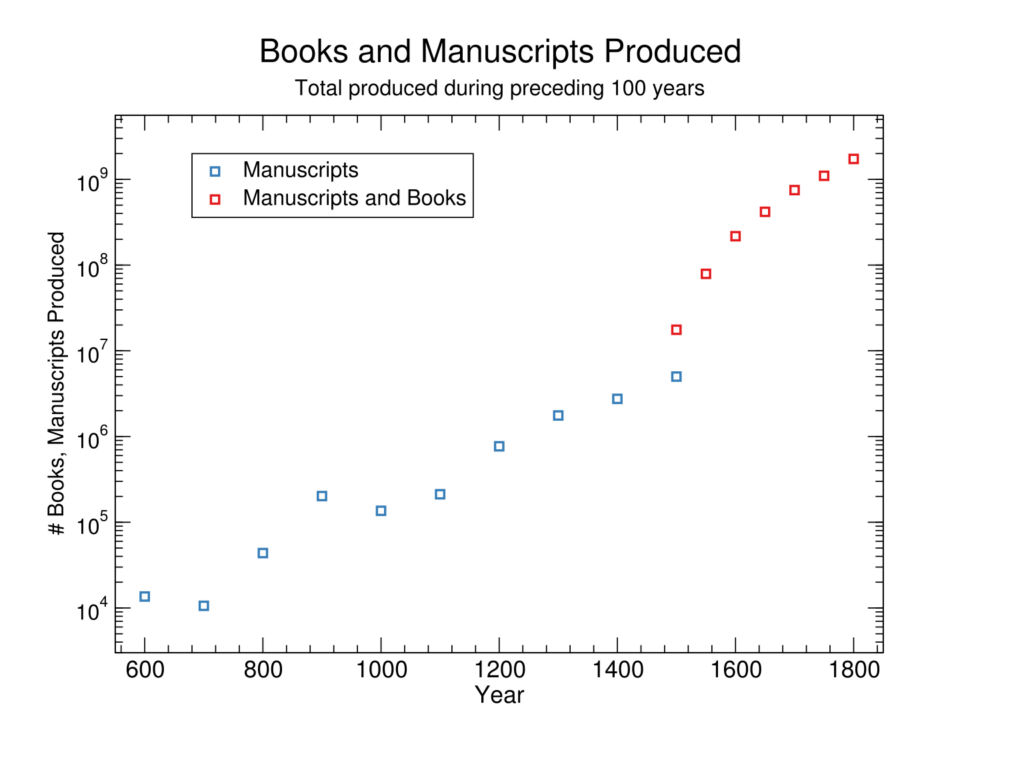
\includegraphics[width=0.8\textwidth]{images_ts/BookProduction.png}
    \caption{The chart shows the number of books created in history. Red dots represent the production after the mechanical printing press invention.} 
    \label{fig:bookProduction}
\end{figure}

\begin{figure}[ht!]
    \centering
    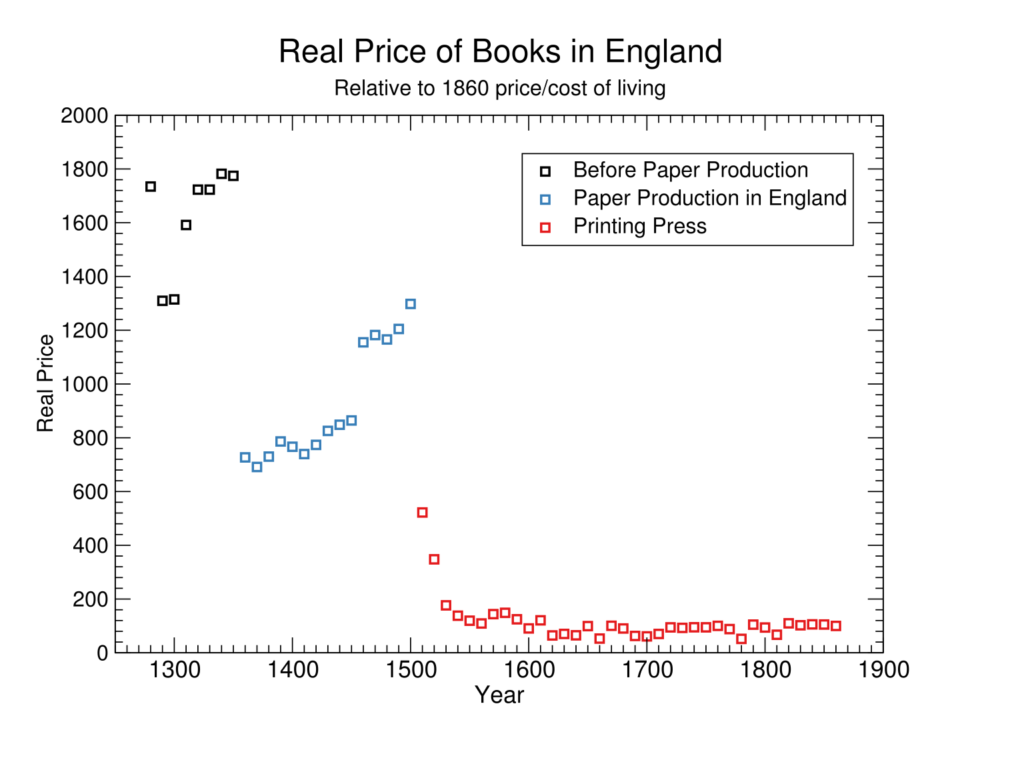
\includegraphics[width=0.8\textwidth]{images_ts/RealPrice.png}
    \caption{The chart shows the price of books in history. Red dots represent the price after the mechanical printing press invention.}
    \label{fig:bookPrice}
    
\end{figure}


\clearpage
\section{Relationship between a stochastic process and a random variable}
In order to get to a more formal definition of stochastic processes, we must first spend some time on theory of probability and define a few terms from this domain.

All the definitions are common for this field of statistics and can be found in many books \cite{time_series_theory}.

\textbf{Def.} If $\Omega$ is a given set, then a $\sigma$-algebra $\mathcal{F}$ in $\Omega$ is a family $\mathcal{F}$ of subsets of $\Omega$ with the following properties
\begin{enumerate}[label=(\roman*)]
\item $\emptyset \in \mathcal{F}$
\item $F \in \mathcal{F} \Rightarrow F^C \in \mathcal{F}$, where $F^C = \Omega \setminus F$ is the complement of $F$ in $\Omega$
\item $A_1,A_2,... \in \mathcal{F} \longrightarrow$ $A:= \bigcup_{i=1}^{\infty} A_i \in \mathcal{F}$
\end{enumerate}

The pair $(\Omega, \mathcal{F})$ is called a measurable space. A probability measure P on a measurable space $(\Omega, \mathcal{F})$ is a function $P: \mathcal{F}\to [0,1]$ such that,
\begin{enumerate}[label=(\roman*)]
\item $P(\, \emptyset ) \, = 0$, $P(\Omega) = 1$
\item $A_i \in \mathcal{F}, P( \, A_i ) \, \geq 0$
\item if $A_1,A_2,... \in \mathcal{F}$ and $\{A_i\}_{i=1}^{\infty}$ is disjoint (i.e. $A_i \cap A_j = \emptyset$ if $i \neq j$) then
\end{enumerate}

\begin{equation*}
    P( \, \bigcup_{i=1}^{\infty}A_i) \, = \sum_{i=1}^{\infty}P(A_i)
\end{equation*}

The triple $(\Omega, \mathcal{F}, P)$ is called a probability space. The subsets $F$ of $\Omega$ which belong to $\mathcal{F}$ are called $\mathcal{F}$-measurable sets. 
Some of possible $\sigma$-algebras
\begin{itemize}
		\item $\mathcal{F} = \{\emptyset,\Omega\}$ is $\sigma$-algebra
		\item for any $A \subset \Omega$ is $\mathcal{F} = \{\emptyset,A,A^C,\Omega\} \sigma$-algebra
		\item $\mathcal{F} = 2^\Omega$ -- here $\sigma$-algebra is produced by all of the subsets. This is the most commmon choice for finite or countable $\Omega$
		\item Borel $\sigma$-algebra $\mathcal{B}$ -- the smallest $\sigma$-algebra which contains all open sets, all closed sets, all countable unions of closed sets, all countable intersections of such countable unions etc. This is the most common choice for uncountable $\Omega \in \mathbb{R}^n$
	\end{itemize}

\textbf{Def.} Random variable $X$ on probability space $(\Omega, \mathcal{F}, P)$ is a function which asigns value $X( \, \omega) \, \in \mathbb{R}$ to every result of experimnt $\omega \in \Omega$. There is important for $X$ to be measurable.
\begin{equation*}
    \{X \leq x\} \in \mathcal{F}, \forall x \in \mathbb{R}
\end{equation*}

\textbf{Def.} Distribution function of the random variable $X$ is defined as below. Distribution function uniquely determines probability distribution of the random variable.
\begin{equation*}
    F_X( \,x) \, = P( \,X \leq x )
\end{equation*}

\textbf{Def.} Random variable $X$ is continuous, if there exists non-negative function $f_X$ such that, $\forall x \in \mathbb{R}$
\begin{equation*}
    F_X( \,x) \, = \int_{-\infty}^{x} f_X( \,t) \, \,dt
\end{equation*}


\textbf{Def.} Expected value of discrete random variable $X$, is defined as
\begin{equation*}
    E X = \sum_{k} x_k P( \, X=x_k ) \, = \sum_{\Omega} X( \,\omega) \,P( \,\omega) \,
\end{equation*}

\textbf{Def.} Expected value of continuous random variable $X$ which density function is $f$, is defined as
\begin{equation*}
    E X = \int_{-\infty}^{\infty} x f( \, x) \, \,dx = \int_{\Omega} X( \, \omega) \, \,d P( \, \omega) \, 
\end{equation*}

\textbf{Def.} Two subsets $A, B \in \mathcal{F}$ are called independent if  
\begin{equation*}
    P( \, A\cap B ) \,  = P( \,A ) \, P( \,B ) \, 
\end{equation*}

A collection of $\{A_i | \quad i: \in I\}$ is independent, if
\begin{equation*}
    P( \, \bigcap_{i \in J}A_i) \,  = \prod_{i \in J} P( \,A_i ) \,
\end{equation*}

Now we can start to define stochastic process within the world of random variables.

\noindent\textbf{Def.} A stochastic process is a parametrized collection of random variables
\begin{equation*}
    \{X_t\}_{t \in T}
\end{equation*}

defined on a probability space $(\Omega, \mathcal{F}, P)$ and assuming values in $\mathbb{R}^n$.
The parameter $T$ is usually the halftime $[0,\infty)$, it can be also an interval $[a,b]$, where $a,b \in \mathbb{R}^n$ for $n \geq 1$. It is important to note that for each $t \in T$ we have a random variable
\begin{equation*}
    \omega \rightarrow X_t(\,\omega )\, \quad       \omega \in \Omega.
\end{equation*}

On the other hand, fixing $\omega \in \Omega$ we can consider the function
\begin{equation*}
    t \rightarrow X_t(\, \omega )\, \quad       t \in T
\end{equation*}

which is called a path of $X_t$.
For the better intuition we may think of $t$ as time and each $\omega$ as an individual experiment. With this picture $X_t( \,\omega) \,$ would represent the value at time $t$ of the particular experiment $\omega$. Because of convenience we can rewrite $X_t( \, \omega) \,$ as $X( \, t,\omega) \,$. By this step we created function of two variables $( \, t, \omega) \, \rightarrow X( \, t, \omega) \,$ from $T \times \Omega$ into $\mathbb{R}^n$. This type of thinking about stochastic processes is very important because now we clearly see that $X( \,t, \omega ) \,$ is jointly measurable in $( \,t, \omega) \,$. Further in text we will use simplified notation as random variable $X_t$ and $x_t$ as it's realization. We may use a simplified notation for the time series as well. This means that we will denote to $Y$ as sequence of measurements. 

\clearpage
\subsection{Time series analysis}
To understand the information, we need to analyse the stochastic process expressed as a time series. We work with a sequence of measurements where each measurement is a realization of a random variable $X$ with index $t$. We can calculate all the characteristic properties of random variable on such a set of measurements.


\textbf{Mean value}
\begin{equation*}
\mu_{t} = \mathbb{E}[ \,X_t ] \,\quad   t \in T
\end{equation*}

\textbf{Variance}
\begin{equation*}
\sigma_{t}^2 = var( \, Y_t )\,\quad t \in T
\end{equation*}

\textbf{Autocovariance}
\begin{equation*}
\gamma( \, t_1, t_2 ) \,  = cov(\, Y_{t_1}, Y_{t_2})\, = \mathbb{E}[ \, ( \, Y_{t_1} - \mu_{t_1} ) \, (\, Y_{t_2} - \mu_{t_2}  )\, ] \,
\end{equation*}

\subsection{Autocorrelation and partial autocorrelation}
We can try to understand how past events influence future events by examining the time series. For that we need a tool to observe how the measurement in the case $X_{t+n}$ is affected by the measurement $X_{t}$.

\noindent\textbf{Def.} Let us assume a time series $Y = \{Y_t |t \in T\}$ with mean $\mu_{t}$ and variance $\sigma_{t}^2$ for each $t$. Autocorrelation coeficient for time indices $t_{1}$ and $t_2$ is defined as 
\begin{equation*}
    \rho_{t_1,t_2} = corr(Y_{t_1}, Y_{t_2}) = \frac{\mathbb{E}[(Y_{t_1} - \mu_{t_1})(Y_{t_2} - \mu_{t_2})]}{\sigma_{t_1} \sigma_{t_2}} \quad \rho_{t_1,t_2} \in [-1,1]
\end{equation*}

\noindent\textbf{Def.} Let us assume a time series $Y = \{Y_t |t \in T\}$. Partial autocorellation lag $k \geq 1$ denoted as $\alpha( \,k)\,$ is autocorellation between $Y_t$ and $Y_{t+k}$ after removing the effect of the linearly intervening variables $Y_{t+1},\dots,Y_{t+k-1}$

\begin{equation*}
    \alpha(k) = \frac{ cov(Y_t,Y_{t+k}|{Y_{t+1}\dots Y_{t+k-1}}) }{\sqrt{
    var(Y_t|{Y_{t+1}\dots Y_{t+k-1}})var(Y_{t+k}|{Y_{t+1}\dots Y_{t+k-1}})}}
\end{equation*}

\newpage
\section{Time series decomposition}

When observing and analyzing a time series, it happens quite often that with expert knowledge or experience from previous observations we know that information is a composition of several properties. The basic properties of a time series include seasonality, trend, cyclical changes and other irregular fluctuations.
\begin{itemize}
		\item \textbf{Seasonality} -- represents a regularly recurring component of the time series. The seasonal component may represent, for example, the alternation of rainy and dry seasons in subtropical areas, the influence of the season on customer behaviour, etc.  
		\item \textbf{Cyclical changes} -- a component that is caused by irregularly recurring changes. This includes events that are several times the size of the observed area. Such events include, for example, long-term changes in the economy, continual evolution of the weather, etc.
		\item \textbf{Trend}  -- in general, it is often defined as the long-term evolution of the mean value.    
		\item \textbf{Irregular fluctuations} 
	\end{itemize}

The components of the time series can be aggregated into one information and represented as the time series ${Y_t}$. There are two types of time series models that are mainly used.

\textbf{Additive}
\begin{equation*}
Y_t = T_t + S_t + E_t
\end{equation*}

\noindent\textbf{Multiplicative}
\begin{equation*}
Y_t = T_t \cdot S_t \cdot E_t
\end{equation*}

where the observed variable is ${Y_t}$, the trend is represented by ${T_t}$, the seasonality is represented by ${S_t}$ and $E_t$ represents the unexplained component. In this component, the irregular fluctuations and the long-term cycles component are merged.

The main difference between the type of model is the processes that we want to describe with the specific model. In additive models, the seasonality of the component hardly changes with increasing time. In multiplicative models, the seasonal amplitude increases gradually with increasing time.

\begin{figure}[ht!]
    \centering
    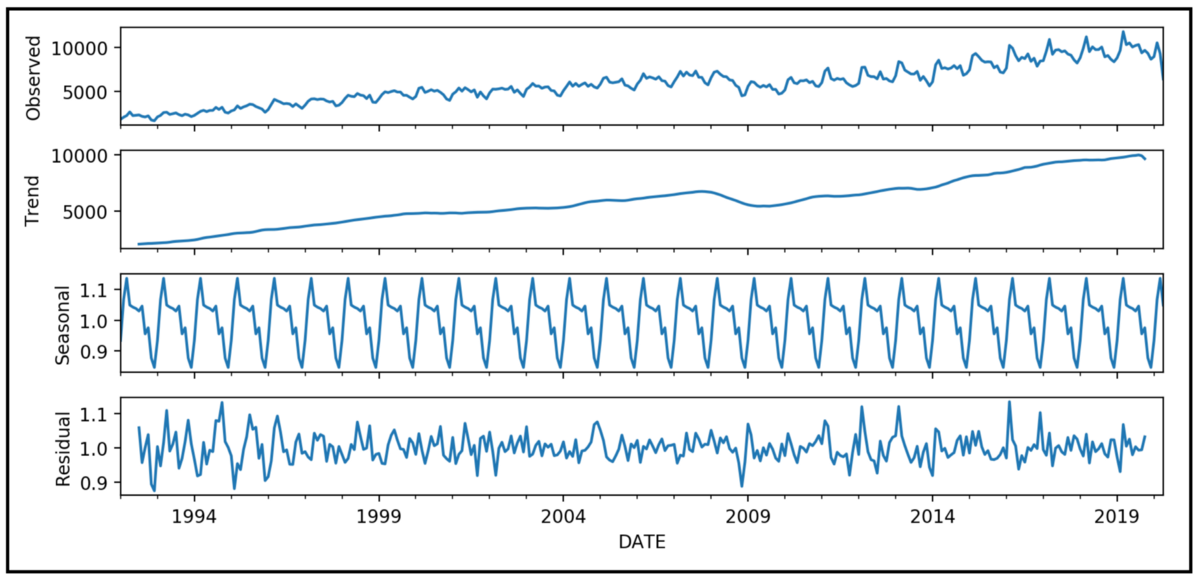
\includegraphics[width=1.0\textwidth]{images_ts/7d100-1mzkkvu_ih6qemb_mz83oaw.png}
    \caption{Components of time series.} 
    \label{fig:residual_conn}
    
\end{figure}

Thanks to such a decomposition of the observed process, we can reveal the presence of a trend, the seasonality, additive or multiplicative character in the initial analysis.
Based on the decompositon we can infer the relationship between the variables and suggest further steps of the analysis which are best suited to the specific problem.
We can further process the time series information and extrapolate from it to make predictions for the future development of the time series.

\subsection{Stacionarity}
Stationarity is one of the characteristic properties of time series. It describes the distribution of random variables over different parts of the time series. 

There are several types of stationarity.
\begin{itemize}
		\item \textbf{Strict stationarity} -- we talk about strict stationarity in the case that the combined distibution $Y_{t_1},\dots,Y_{t_k}$ is the same as the combined distibution $Y_{t_1 + \tau },\dots,Y_{t_k + \tau}$ for $\forall t_1, \dots, t_k, \tau$. If this condition is satisfied then the stationary series is strictly stationary.  
		\item \textbf{Weak stationarity} -- we talk about weak stationarity if the time series is invariant with respect to time shifts in moments to second order $\mathbb{E}[Y_t] = \mu$ and $cov(Y_t, Y_{t+\tau}) = \gamma(\tau)$.
	\end{itemize}

Strict stationarity is often very restrictive. That is why weak stationarity has been introduced.

\chapter{Tools exploration}
\label{label:Useful_tools}
In the following chapter we explore the tools and approaches that can be used to retrieve information and data from repositories.

\section{Criteria for selection}
From the beginning of the work on the assignment, we focused on the analysis of a large amount of data. It was necessary to get meta information about as many repositories as possible. We needed as much data as possible because we had to go through a set of experiments where we tried to train smaller models on subsets of different parts of the dataset. 

We had to get the data first. We didn't know in advance which data contained the information needed to predict the lifetime of the repository. That is why it was vital that we were able to repeat this process of obtaining repository information multiple times at a reasonable speed. If this process takes too long it is very difficult to train the model. The quality of the model is very closely related to the quality of the input data.

At this stage of the project, we could have proceeded in several ways to acquire the data. Some were more direct and at first glance looked like a quick win. Others assumed the use of 3rd party tools, which would limit the collection to a certain extent in terms of diversity, but also speed it up in case we want to get very concrete and specific information already from the indexed database. 

\section{GithubAPI}
The first choice to get the data was to use a tool that Github provides directly. It is very well adapted to work with the repository. Developers use it to make working with the repository faster and easier.  Thanks to the exposed API, it is possible to get any information, for example, commit history, file size, status of tests of the last version of the product, number of stars, etc. The API provides several thousands of functions that cover the needs of developers.

However, we did not want to use the API exactly as it was originally designed. We needed to get information from as many repositories as possible. It was not enough to just download the information. There was no need to set up specific nuances for one particular repository. Rather, we wanted to access more generic information such as commit history, files with different suffixes, readme files, etc. It was important that we had to be able to do this quickly.   

When working with the API, you could feel the focus with which the Github team built it. It is supposed to be used for detailed management of just one repository. 

The emphasis was also on speed. The x-rate-limit variable is incremented when the API is called. This variable limits the number of calls quite strictly.  For unauthenticated users the limit is 60 calls per hour. If the API is used by an authenticated user, the limit is 5000 calls per hour.

The limit was a strict restriction. That is why we decided to use GithubAPI as one of the tools and not as a standalone solution.

\section{Github Archive}
The solution works as an event listener that gets information on a periodic basis and stores it in the database. The collection of information is taken care of by an event listener that scans the Github global timeline every hour. It stores this information in JSON format in a document DB. A user is able to get a db snapshot and work with the data offline.

The data is also preprocessed and persisted to a SQL like database. The database is accessible via BigQuery.

\section{GHTorrent}
An alternative to Github Archive. Data collection and persistence works analogously. To access MongoDB where the information is uploaded you need to upload a personal access key to the GHTorrent repository. Then the user gets access to MongoDB. Access to BigQuery is not conditional on anything. Since GHtorrent has been a deprecated project for some time, the pull reguest to upload the key was not successful.
A user is able to get a db snapshot and work with the data offline.

Nevertheless, we decided to use this tool. Its biggest contribution is in its one detailed relational model. The structure in which the repository information is stored suited our needs very well.

The information database is not updated regularly. But that didn't bother our usecase at all.

\section{Other alternatives}
We have decided to mention a couple of other alternatives. These tools are very efficient when it comes to retrieving information from a small number of repositories. They were not suitable for our usecase.

\begin{itemize}
		\item AskGit -- SQL like command line tool. Very restrictive as far as the relational model is concerned. For our usecase this solution was not suitable.
		\item CHAOSS -- a visualization tool that allows you to display information about the community, repositories, etc. It contains a set of tools that can be customized and adapted to your needs to a certain extent. It belongs to the family of tools that deals with source code management - data mining, analytics, visualization.
		\item SourceCred -- a tool that creates a collaboration graph where nodes are user, commit, issue, author, etc. and edges represent relationships between them.
		\item Sourced -- the solution contains several interesting instruments. For example Hercules, which works very efficiently with the overall commit history. Gitbase allows to work with the repository using sql query language.
	\end{itemize}

\chapter{Data acquisition}
\label{label:Data_acquisiton}
In this chapter we discuss different approaches taken during work with dataset. We proceed to a fast iterative cycle. Thanks to this we are able to find relevant information. Based on information from this data, we later train the models. We discuss working with the dataset, its acquisition, processing, cleaning. In the last part we discuss the creation of a generator that serves the models during training.

\section{Tools suitable for usecase}
We have researched several tools that solve data acquisition process. This was the very first step which if neglected can complicate the solution. We wrote about these tools in \ref{label:Useful_tools}. Each one of them had its own advantage. Most of them focused on working with individual repositories, but this is not our case. We decided to use GithubAPI together with GHTorrent. GithubAPI has a huge added value. users are able to query a detailed missing information about the repository. GHTorrent serves as a place where we can find a large amount of structured data that would be very hard to get without it.

\begin{figure}[ht!]
    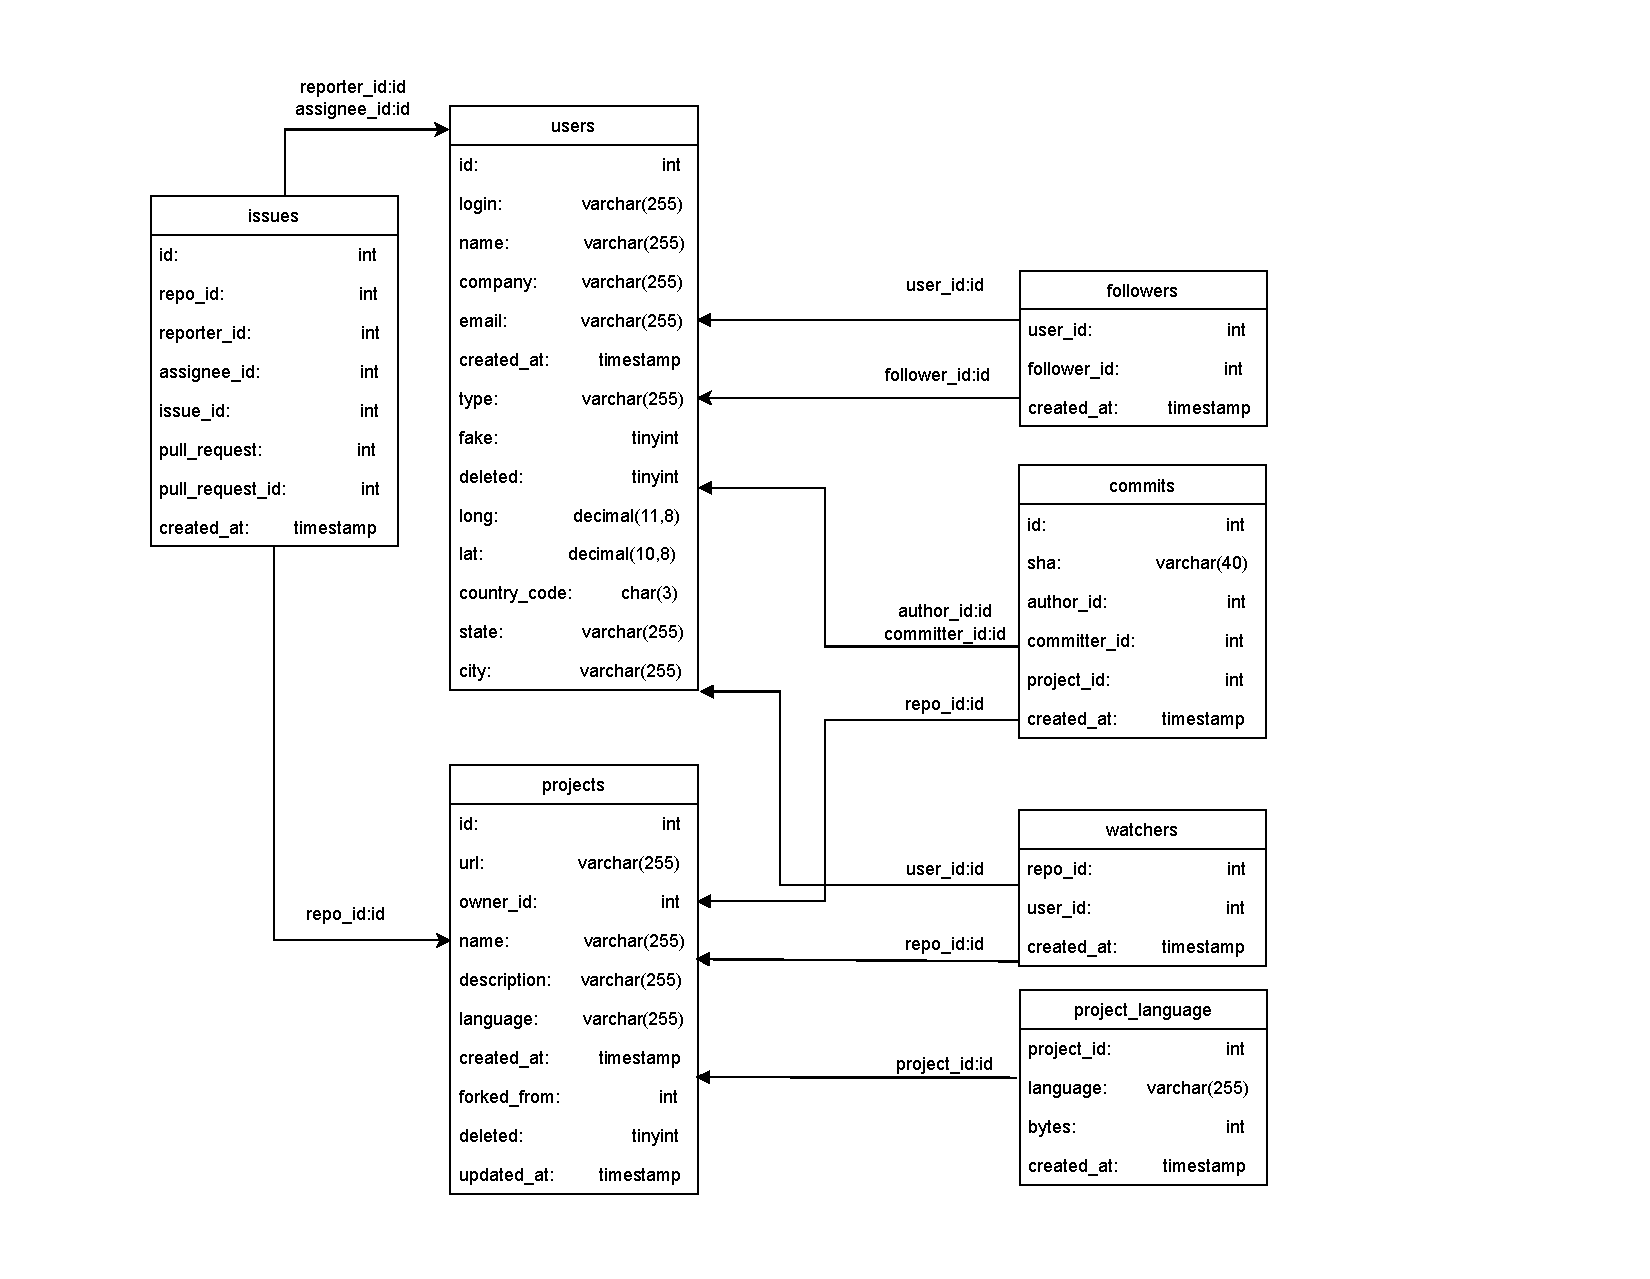
\includegraphics[height=0.6\textheight]{images_ts/diag.drawio (1).pdf}
    \caption{Entity model shows which entities from the GHTorrent schema we worked with.} 
    \label{fig:relation_in_data}
    \centering
\end{figure}

There are several mysql database dumps with information about repositories on GHTorrent. The first dump is from 2013. As the project grew in popularity, so did the intensity of data collection. Over the last period of time the project has gotten to a less supported state. The author runs the data collection script very sporadically. The last dump used by us was collected on 2021-03-06. We experimented with uploading part of the data to a local station. It was possible to upload the table of users and repositories on a local pc/low tier pc on AWS. If we wanted to upload commit table from dump, the processing time and space needed to store the information was unbearable. The author of the last dump uploaded it to BigQuery. Thanks to that we could work with the data in a reasonable way.
\newpage
\section{Exploratory data analysis}
\label{label:Exploratory_data_analysis}

\subsection{Overview}
The first experiments were with repositories written in python. We managed to filter such repositories very easily because the relational schema contains a table that has the language attribute.

We selected a random sample of 10000 repositories that we wanted to examine. Our task was to find such metadata in the repositories that could be used to predict the lifetime of the repository. 

By successive examination of the data we obtained several candidates whose information could correlate with the activity of the repository. 

\subsection{EDA in detail}
As we were examining the smaller sample set, we realized a few facts. We were looking at a random sample of repositories that didn't really yield any information. Our findings led us further and further away from our goal.   

About 80\% of the repositories were rarely ever active. Such repositories were projects that people cloned but never worked on, small experimental projects that eventually led nowhere, various AI courses, etc. Any information about such repositories was irrelevant \ref{fig:zero_commits}. For the ML model, which relies on quality data and well processed data, it was counterproductive.

\begin{figure}[ht!]
    \centering
    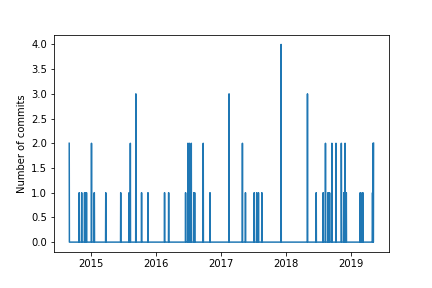
\includegraphics[width=0.8\textwidth]{images_ts/zero_commits.png}
    \caption{Commit activity during the year. This is what a average repository looked like. For a large part of the year, there is nothing to see even if we aggregated the activity by month.} 
    \label{fig:zero_commits}
\end{figure}

We had to get rid of these repositories. But the cleanup process had to be approached carefully. When amputating data, we had to get rid of the unwanted part of the dataset without damaging the part that contains relevant information for training the model. We were able to keep the relevant repositories thanks to aggregating the number of unique users in the repository. Empirically, we set the value to 5. We consider all repositories on which at least 5 unique users collaborated. Using this modified query, we obtained a new sample of repositories from BigQuery.

Even after these modifications, the repositories still has not reached the quality we needed. When displaying information about randomly selected data points, they are very diverse and inconsistent. We want to predict the lifespan of repositories that represent some community-supported tool, some package or library. 

The data still contained data points that even a well-trained model would not be able to deal with well. It was necessary to figure out a way to filter out at least a larger part of the repositories that are not covered by the focus of our usecase. But such information that we could have used for filtering was not present directly in the data yet. 

Many of the attributes we wanted to investigate were only accessible via GithubAPI (e.g. whether a repository belongs to an organization, number of stars, etc.).  The speed of data retrieval for the experiment was quite limited. Maximum 5000 requests per hour. We managed to get a couple of additional access tokens "from family and friends". Thanks to that we created a set of functions using async.io library that can work with GithubAPI incomparably faster than the naive solution. This has helped examined a much larger set of candidates.

We have experimented with a number of attributes that could have been used to filter the repositories. We always aggregated the information based on some attribute and then displayed how the distribution looks like over the whole dataset. It was important to normalize the values and compare the normalized values. For example, a large repository may have a large number of users but the average number of commits per user is small. This brought us to a scale where we could compare all repositories. After a few experiments a candidates emerged.

The size of the \ref{fig:size_of_repos} repository turned out to be a reasonable indicator, thanks to which we can filter other repositories. But we could not get this information from GHTorrent. We were able to get it from GithubAPI.

\begin{figure}[ht!]
    \centering
    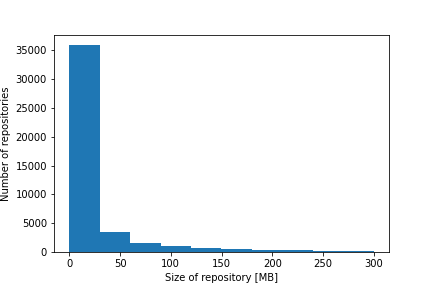
\includegraphics[width=0.8\textwidth]{images_ts/size_of_repos.png}
    \caption{Uneven presence of repositories of different sizes. Smaller repositories clearly predominate.} 
    \label{fig:size_of_repos}
\end{figure}

We have filtered out repositories of smaller size. Thanks to this we got a list of repositories that are good candidates for model training.

\clearpage
\section{Dataset}
\label{label:Dataset}
\subsection{Multivariate time series}
After data processing and extensive EDA, we decided to keep information about commit history, number of issues created and number of followers in the dataset. We created a subset of time series from each data point describing the activity in the repository.  

\ref{fig:multivariate}.

\begin{figure}[ht!]
    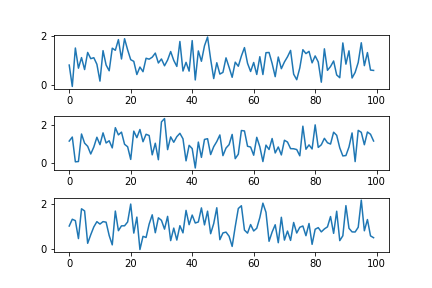
\includegraphics[width=0.8\textwidth]{images_ts/multivariate.png}
    \caption{The graph shows a general multivariate time series task. Each sub graph represents one of observed variable.} 
    \label{fig:multivariate}
    \centering
\end{figure}

We have managed to filter out the repositories we will not be working with. We had to prepare this set for training. For example, a time series describing commit history looks like an inactive repository at low resolution. If we take a look on the activity graph, there would be zero values most of the time.

\subsection{Sparse time series}

If the measured process has zero values for most of tme observations, then we talk about sparse time series.

Models based on LSTM architecture have a hard time predicting such a sparse time series. Occasional zero values would not be an obstacle. The problem is if 90\% of the time series information is zeros. Model will not work properly. We have seen this in an experiment. After training on such sparse data, the model was not able to classify the lifetime of the repository. 

We decided to use a larger time window and aggregate the information at 7, 14,30 and 60 days. Aggregation at the 30 day level was the most suitable. Then we partially got rid of the zeros but the parts when the repository is actually inactive remained unaffected by our modification.


\begin{figure*}[ht!]
    \centering
    \begin{subfigure}[t]{0.5\textwidth}
        \centering
        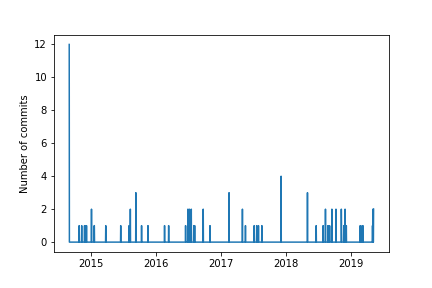
\includegraphics[width=1.0\textwidth]{images_ts/zero_commits_agregated_days.png}
        \caption{Time series commits intensity aggregated by day.}
    \end{subfigure}%
    ~ 
    \begin{subfigure}[t]{0.5\textwidth}
        \centering
        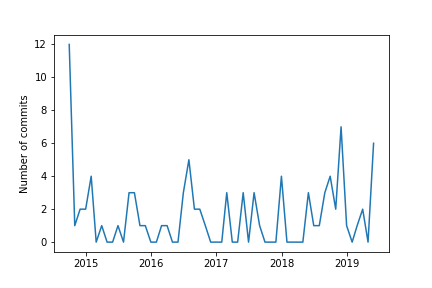
\includegraphics[width=1.0\textwidth]{images_ts/zero_commits_agregated_months.png}
        \caption{Time series commits intensity aggregated by month.}
    \end{subfigure}
    \caption{Different types of aggregation intervals. Larger window suits the models much better.}
\end{figure*}

\subsection{Repository life cycle}
Before the work started, we were looking for a dataset that could serve us. We have not found a similar one that we needed for our task so we had to create one. The main requirement was to be able to classify the lifetime of the repository based on its historical activity.

To be able to predict where a repository becomes inactive, we had to work with repositories that have gone through a full life cycle. From early activity to gradual decadence and subsequent inactivity. 

\begin{figure*}[h]
    \centering
    \begin{subfigure}[t]{0.5\textwidth}
        \centering
        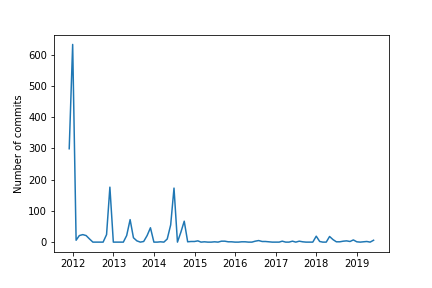
\includegraphics[width=1.0\textwidth]{images_ts/repo_rising_decling_dead.png}
        \caption{The entire life cycle of a repository.}
        \label{fig:repository_whole_life_cycle}
    \end{subfigure}%
    ~ 
    \begin{subfigure}[t]{0.5\textwidth}
        \centering
        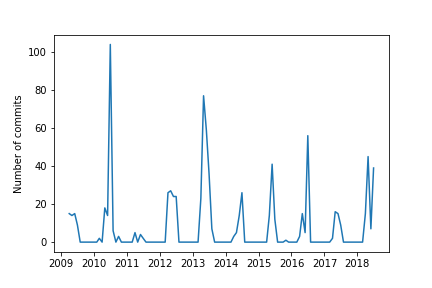
\includegraphics[width=1.0\textwidth]{images_ts/repo_rising_still_active.png}
        \caption{Repository which is still active.}
    \end{subfigure}
    \caption{A repository that has gone through its entire life cycle can be used for training models. A repository that is still active must be filtered out from the training set.}
\end{figure*}

The repository whose entire life cycle we have documented is in the image \ref{fig:repository_whole_life_cycle}. Similar looking datapoints will help us to train the classification model.

Looking at the pictures, it is obvious when the users stopped being active in the repository. This information should have been included in the training data. For repositories, we considered the end of activity to be the point in time t where the average activity in the next 12 months did not go over 5\% of the highest activity in the repository. We will further assume time t to be the end of repository lifetime.

\newpage
\subsection{Training data generator}
\label{label:training_data_generator}
After all the editing and cleaning we had to create the data for training. Since we want to augment the time series during the training process, we decided to create a data generator.

Based on the information when the repository became inactive, it can generate a time series of the corresponding length and the corresponding label. 

The generator works with the original time series. It works with values $x_{t_0},\dots,x_{t_n}$, where $t_k \in {[24,\dots,n-1]}$ represents the number of months since the beginning of the repository's existence. Therefore, the minimum activity of a repository must be at least 24 months. The upper limit is the point where it became inactive. If the value $t - t_k$ (the distance of the current date from the date when the repository is considered inactive) is more then 12 months, then the repository is considered active otherwise it is inactive. 
We work with multivariate data. The generator had to be adapted to this fact.

Let us assume dataset $\{{(x_1,y_1), (x_2,y_2),\dots,(x_n,y_n)}\}$, where $x_k\in$ $\mathbb{R}^{v \times l}$, where $v$ represents number of examined time series, $l$ represents length of time series and $y_k \in \{0,1\}$. 
\chapter{Time series classification}
\label{label:Timeseries_classification}
This chapter deals with a large number of approaches used in time series analysis. It describes their theoretical foundations. Each section is devoted to a specific algorithm. We focus on the process by which the algorithm processes the time series and then classifies it. The chapters discuss the advantages and disadvantages of the individual approaches.

\section{Time series classification algorithms}
Problems requiring processing and subsequent analysis of time series are encountered quite often in machine learning practice. Solved problems and tasks always have a slightly different characteristic and so a large number of models and approaches have been developed to analyze and classify time series.
Among the main approaches belong, for example

\begin{itemize}
		\item Nearest neighbour 
		\item Kernel methods
		\item Shapelet-based approaches
		\item Tree-based approaches
		\item Bag-of-words approaches
		\item Markov transition field
		\item Deep learning
	\end{itemize}
\subsection{Nearest neighbour}
The algorithm of nearest neighbours compares the samples. Based on the comparison, it determines the final class of the observed sample. Thus, the classification of a sample is decided by its nearest neighbours. Different metrics are used to measure similarity. The most common is the Euclidean norm.

This approach of measuring the similarity between samples of different data is sufficient. However, it has a set of disadvantages when comparing data of a temporal nature and is not very suitable for such a task.
\begin{itemize}
		\item The first disadvantage is the size of the compared pair of time series. The Euclidean metric only works with 2 vectors of the same size. Time series often have variable length.
		\item The Euclidean metric treats the values of each vector as independent variables. This assumption is not satisfied for time series because often the current value depends on the previous one. In other words, the values of the time series are auto-correlated.
	\end{itemize}
\subsection{Nearest neighbour without modifications}
These shortcomings can be observed, for example, in a tourist application that records the movement of tourists. Let 2 hikers walk along the same hiking trail and record their altitude. They are walking on similar terrain so we assume that the time series of the recorded information will be almost the same. But Euclidean distance cannot reveal such similarity. The model situation is, for example, when one hiker walks a given route faster than the other. Then the time series describe the same process but the length of the vectors is different as well as obtained data differs. In such a case the comparison using Euclidean distance cannot be used.

It is for the above reasons that the Dynamic time warping algorithm was developed. It solves both of problems.
\subsubsection{Dynamic time warping}
\label{label:Dynamic_time_warping}
Dynamic time warping was developed mainly for time series comparison in speech recognition. It generates optimal global alignment between two time series, expoiting temporal distortions between them. The algorithm computes a cost matrix that minimizes the difference between the values of the two time series. At the end, the algorithm reconstructs a path that represents the best mapping between the points of the two time series.

\noindent Let $X = (x_1, \dots, x_n)\in \mathbb{R}^n$ and $Y = (y_1, \dots, y_m) \in \mathbb{R}^m$ be two time series.
Then the cost matrix between these two time series is defined as
\begin{equation*}
    \forall i,j \in \{1,\dots,n\} \times \{1,\dots,m\}, C_{ij} = f(x_i,y_j)
\end{equation*}
We use the Euclidean metric to measure the distance between the points of the time series.

\noindent A warping path is a sequence $p = (p_1,\dots, p_L)$ such that
\begin{itemize}
		\item value condition: $\forall l \in \{1, \dots ,L\}$, $p_t = ( i_l,j_l) \in \{1,\dots,n\} \times \{1,\dots,m\}$  
		\item boundary condition: $p_1 = (1,1)$ and $ p_L = (n,m)$
		\item step condition: $\forall l \in \{1, \dots ,L - 1\}$, $p_{t+1} - p_t \in  \{(0,1), (1,0), (1,1)\}$
	\end{itemize}

Cost of warping path for both time series is
\begin{equation*}
    C_p(X,Y) = \sum_{l=i}^{L}C_{i_l,j_l}
\end{equation*}

The dynamic path score is defined as the minimum cost among all the warping paths
\begin{equation*}
    DTW(X,Y) = \min_{p \in P} C_P(X,Y)
\end{equation*}
where $\mathcal{P}$ is the set of all warping paths. We can use dynamic programing to decrease the complexity of computation. The complexity of problem decreases to $\mathcal{O}(nm)$. The difference between two consecutive elements of warping path can be computed as
\begin{equation*}
\begin{split}
    DTW(X_{:i},Y_{:j}) = C_{i,j} + min\{ & DTW(X_{:i-1},Y_{:j-1}), \\ 
    & DTW(X_{:i-1},Y_{:j}), \\ 
    & DTW(X_{:i},Y_{:j-1})\}
\end{split}
\end{equation*}

\noindent We can define accumulated cost matrix as
\begin{equation*}
\forall i,j \in \{1,\dots,n\}\times\{1,\dots,m\}, D_{i,j} = DTW(X_{:i},Y_{:j})
\end{equation*}

% \noindent to be able to compute accumulated cost matrix in dynamic fashion we need to initialize it's first row and column with it's cumulative values
% \begin{itemize}
% 		\item $\forall j \in \{1,\dots,m\} D_{1,j} = \sum_{k=1}^m C_{1,k}$
% 		\item $\forall i \in \{1,\dots,n\} D_{i,1} = \sum_{k=1}^n C_{k,1}$
% 		\item $\forall i,j \in \{2,\dots,n\} \times \{2,\dots,m\} D_{i,j} = C_{i,j} + min\{D_{i-1,j-1}, D_{i-1,j}, D_{i,j-1}\}$
% 	\end{itemize}

\newpage
\subsubsection{Constraints of algorithm}
Like all approaches, DTW has its disadvantages.
\begin{itemize}
		\item Computational time complexity - the DTW algorithm works with two time series of length m,n. The computational complexity of alghoritm is $\mathcal{O}(nm)$ which is very restrictive for longer time series.
		\item DTW is not a metric - the DTW algorithm calculates the similarity between the points of the time series during its run. Metric is non-negative real-valued function. One of the axioms of the metric function is $d(x,y) = 0 \Longleftrightarrow x = y$. In the case of DTW, there may be a case where we are work with different time series but their distance is 0.
		\item Triangle inequality is not valid - we use DTW algorithm to be able to compare two time series. DTW is not a metric so we can not use data structures such as M-tree which is suitable for fast comparison of data points.
		\item DTW is not differentiable - this prevents us from optimizing the loss function using gradient methods.
	\end{itemize}


\subsubsection{Variants of dynamic time warping}
Due to the shortcomings of the DTW algorithm, improvements that try to solve the specific problem has been made.

The first way is to replace the minimizing function with a function that is differentiable. The authors in \cite{soft-DTW} presented a solution using soft-DTW. This modified function can be used as an objective function which is optimized by gradient methods.

Another way to improve DTW is to prevent too long time warping regions. This is achieved by limiting the size of the region of points to which one particular point is compared. 

If the size of the region is limited to size 1, only the diagonal is calculated when calculating the cost matrix. Then the algorithm can achieve time complexity up to $\mathcal{O}(max(n,m))$.

In \cite{Sakoe_and_Chibu} the authors proposed a solution that uses a region size strictly smaller than $\frac{max(m,n)}{2}$. In \cite{Itakura} the authors work with dynamic window size. This varies according to the relative position of a point in the time series. The size of the region is smallest at the beginning and end of the time series. Region size is the largest when algorithm works with the data exacly in the middle of time series. 

\begin{figure}[ht!]
    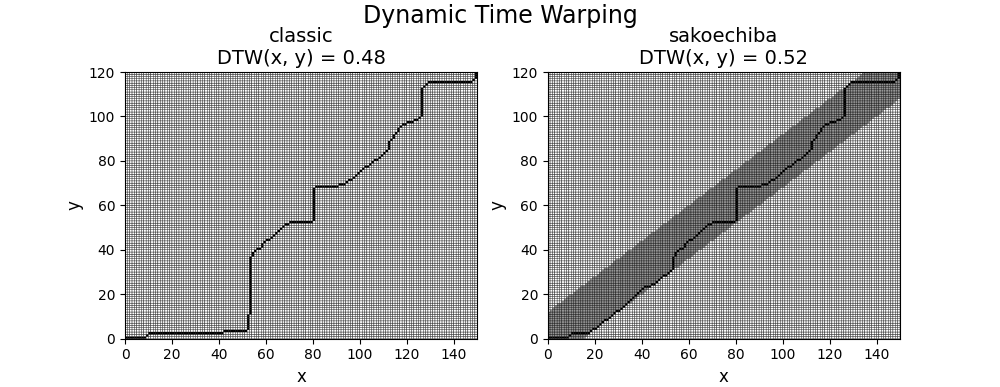
\includegraphics[width=1.0\textwidth]{images_ts/dynamic_time_warping.png}
    \caption{If we use classical DTW, we access all cells of the matrix during the calculation. When using sakoechiba the region is limited. \cite{DTW_optimization}}. 
    \label{fig:dynamic_time_warping}
    \centering
\end{figure}

\subsection{Kernel methods}
In the real world, we often encounter data that is not linear in nature. We cannot explicitly create a linear model such as support vector machines that decouple data using a hyperplane. In a non-linear space, we need to use more sophisticated models and methods to understand the dependencies between data.

By using the kernel we can work with non-linear data and at the same time we can use approaches and models that assume linear data as the input.

The basic idea is to go into the space in which we can make the dot product of transformed vectors efficiently. If we can write the mathematical operations using the kernel function, we never have to explicitly calculate over the space of the huge dimension \cite{kernel_theory}.

Suppose we have a dataset $\{{(x_1,y_1), (x_2,y_2),\dots,(x_n,y_n)}\}$, where $x_i$ corresponds to data point and $y_i$ corresponds to label.
We need to define similarity measure in $X$ so we can separate datapoint. This is taken care of by the kernel function
\begin{equation*}
\begin{split}
& k: X \times X \rightarrow \mathbb{R} \\
& (x_1, x_2) \mapsto k(x_1,x_2)
\end{split}
\end{equation*}

satisfying for all $x_1, x_2 \in X$.

\begin{equation*}
k(x_1,x_2) = \langle \Phi(x_1),\Phi(x_2) \rangle
\end{equation*}

where $\Phi$ maps into some dot product space $\mathcal{H}$ called feature space. The similarity measure k is called kernel and $\Phi$ is called kernel's feature map.

A very important requirement for kernel methods is that we want them to be positive definite. This leads to very interesting properties. For example, there are positive definite kernels that can be computed efficiently even though $\Phi$ maps vectors to a space of infinite dimension \cite{kernel_theory}.

DTW is not guaranteed to be positively definitive because it is not a metric. This problem was solved by the authors of \cite{Cuturi}. In the paper they presented a positive definite kernel for time series.
\begin{equation*}
k_{GA}^{\gamma} = \sum_{p\in \mathcal{P}} exp(-\frac{C_p(X,Y)}{\gamma})
\end{equation*}

where $C_p(X,Y)$ is warping path cost, $\mathcal{P}$ is set of all possible warping paths and $\gamma \geq 0$ is smoothing parameter.

The computational complexity while using kernel is $\mathcal{O}(nm)$.

Support vector machines with this propossed kernel yeilds better results that implementations where the limitation of positive-definitness was not satisfied.


\subsection{Shapelet based approach}
Although nearest neighbours algorithms are relatively straightforward and simple to implement, they have their drawbacks. As we saw in \ref{label:Dynamic_time_warping}, nearest neighbor algorithms require storing and searching the entire dataset, which negatively affects the running time of the algorithm. Another drawback is the relatively poor explanatory power of the inferred conclusions from the data. Shapelet based algorithms try to solve these problems.

Shaplets are specific parts of the time series that are characteristic for it. Based on the speciffic characteristic features we are able to better classify the time series. 

In comparison with previous methods, saplets can provide a number of advantages.
\begin{itemize}
		\item Shaplets can provide greater interpretability of classification.
		\item They are more robust and resistant to noisy data. In the leaf dataset they were very capable of classification despite the insect biting the edge of the leaf.
		\item They are faster then algorithms based on DTW. Time complexity of shaplet creation is $\mathcal{O}(ln)$. While working with DTW we need to compare two time series as well as to find the closest neighbour. Time complexity in this case may reach $\mathcal{O}(kn^3)$.
	\end{itemize}


\begin{figure}[ht!]
    \centering
    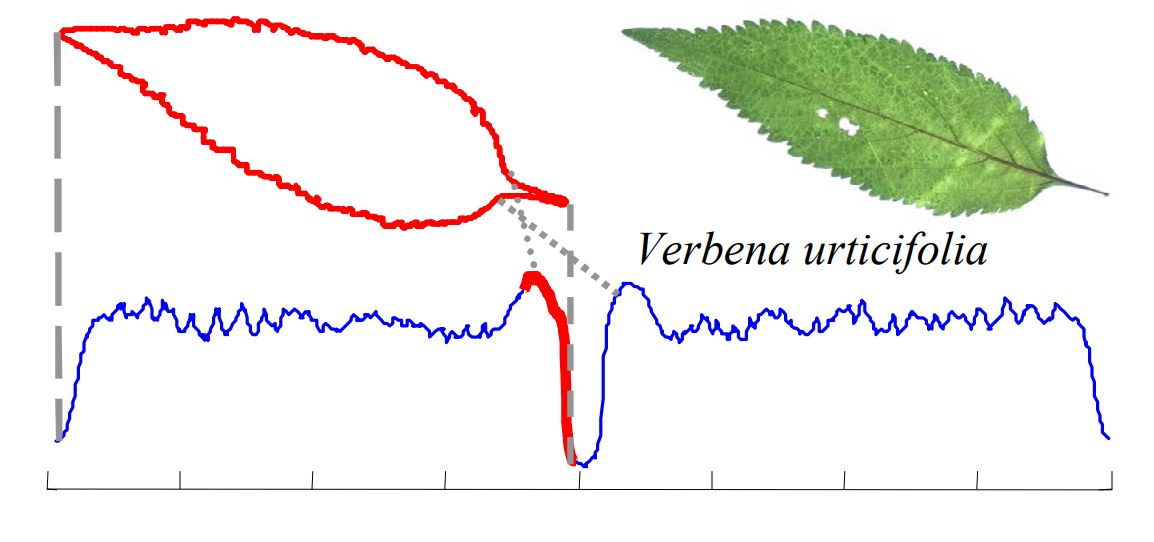
\includegraphics[width=0.8\textwidth]{images_ts/Shaplet_leaf.JPG}
    \caption{The perimeter of the leaf can be represented as a time series. Then the area where the leaf passes into the stem has a specific character. Such a part of the object is identified as a shaplet\cite{learning_shaplet_leaf_img}.}. 
    \label{fig:shaplet_picture}
\end{figure}

\subsubsection{Extracting shaplets}
Let $X = (x_1, \dots, x_n)$ be our time series and $S = (s_1,\dots ,s_l)$ be a shaplet of $l$ values, $l\leq n$. Distance between time series $X$ and shaplet $S$ is calculated as minimum squared Euclidean distance $d(S,X)$ between $S$ and all of other sequences of length $l$ from $X$

\begin{equation*}
d(S,X) = \min_{j \in \{0,\dots, n-l\}} \sum_{i=1}^{l}(s_i - x_{i+j})^2
\end{equation*}

The algorithm returns all existing shaplets in a time series of length $m$. The shaplets are further evaluated based on the F-statistic. The statistics calculates the variance between different classes but also the variance within a class. This step is important because we want to find shaplets that are discriminative for one class. If a shaplet is similar to another shaplet it is discarded from the candidate set.

After identifying the $l$ best shaplets, we can use them to generate new discriminative features. Then the generated features can be used as input for any classification model.

This algorithm has time complexity $\mathcal{O}(Nm^2)$, where $N$ is the number of time series and $n$ is the length of the time series. Another disadvantage is that the minimum is searched using the Euclidean distance. In \ref{label:Dynamic_time_warping} we discuss the drawbacks of the Euclidean metric which we replace with another function.

\subsubsection{Learning shaplets}

Shaplet transformation has one small drawback. Among all possible shaplets, it searches for one that has $d(X,S)$ minimal. Such an objective function is not differentiable and cannot be optimized using gradient methods. Therefore, logistic regression is used whose input is a minimizing function. In this way, logistic regression learns to identify specialized shaplets for a particular class.

\begin{figure}[ht!]
    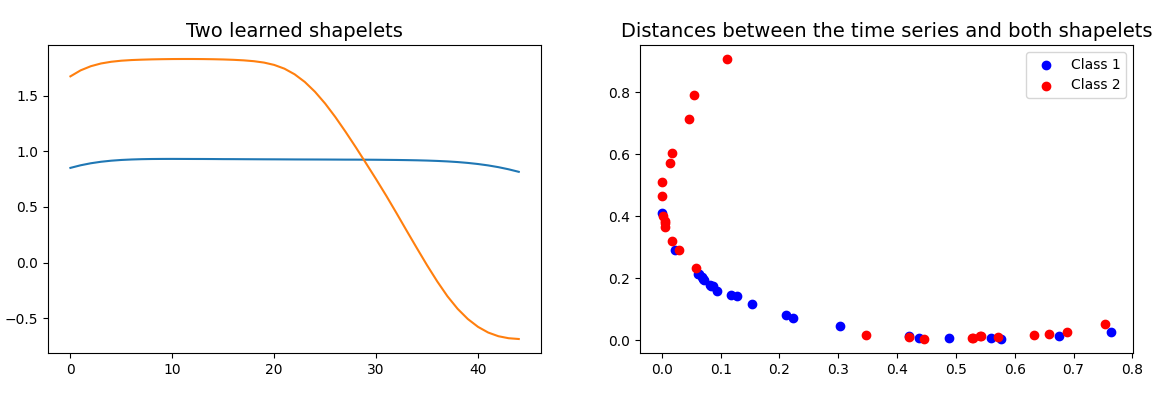
\includegraphics[width=1.0\textwidth,left]{images_ts/learning_shaplets.png}
    \caption{The orange curve contains a common characteristic for a portion of the data. The orange shaplet specifically describes Class 2. The blue shaplet does not carry any specific information about neither of the two classes.\cite{learning_shaplet_img} }
    \label{fig:shaplet_picture_learinng}
    \centering
\end{figure}

\newpage
\subsection{Tree based approach}
Algorithms based on tree methods use very often ensamble approach when classification is not done by one tree but by many smaller trees. This set of smaller models is called a forest.
\subsubsection{Time series forest}
The time series forest algorithm classifies a time series based on information from its subsequences \cite{timeseries_forest}. The hyperparameter $n$ represents the minimum length of a time series subsequence.

Based on the hyperparameter, a set of subsequences is generated and they are further processed. Each subsequence is assigned a mean, variance and slope.

In training, this triplet of attributes is calculated for each generated segment. The triple is then used as input for the classification model.

\subsubsection{Proximity forest}
To better understand the concept of \cite{proximity_forest} proximity trees, we first need to look at the extremely randomized trees algorithm \cite{extreme_random_forest}.
As with training a random forest, several independent trees are trained on the data.The only difference between proximity trees and a random forest is the computational intensity of the selection of the features and the threshold. In a random forest, the information gain (Gini index, Entrophy) is computed in the node of each tree and the data is partitioned according to the features that best partition them.

Proximity forest works with featuresas well. The difference is between computing the treshold. When wokring with poroximity forest then each node generates thresholds randomly for each feature. We try to get as close as possible to this randomly generated threshold with our features. The feature that divide data in best way possible, according to generated threshold, wins. Based on this, the splitting process is much more randomized and much faster compared to normal randomized trees.


The proximity tree algorithm works similarly as the randomized tree algorithm. In a standard tree, the splitting criterion of a node is the feature and the threshold for the given feature. In a proximity tree, it is the metric and the set of instances. The metric is used to compare the similarity of the exemplars. 
As with the extreme random forest, we will have to randomly choose.

\begin{itemize}
		\item For the metric, the algorithm selects from 11 metrices suitable for measuring the similarity of exemplars within a node.
		\item We need to select just one time series from the data. This one data point has a classification class assigned to it. We will compare the other time series to this time series and find out their similarity.
	\end{itemize}

We generate several such pairs and the one that best divides the set of data points is selected as the splitting criterion for our node.

Because a tree with increasing levels reduces the number of unranked data points per node exponentially, it is very well applicable to big data.

\begin{figure*}[ht!]
    \centering
    \begin{subfigure}[t]{0.5\textwidth}
        \centering
        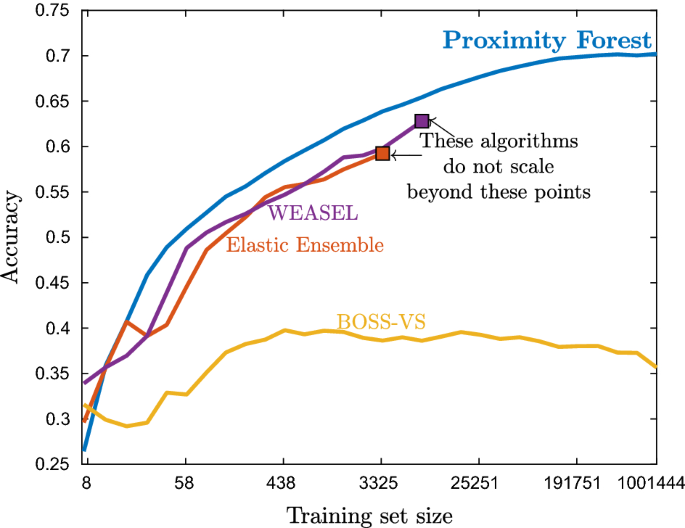
\includegraphics[width=1.0\textwidth]{images_ts/proximity_forest_accuracy.png}
        \caption{Classification accuracy as a function of the size of the dataset \cite{proximity_forest}.}
    \end{subfigure}%
    ~ 
    \begin{subfigure}[t]{0.5\textwidth}
        \centering
        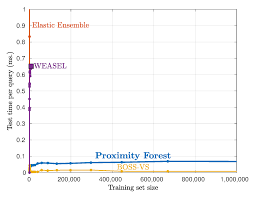
\includegraphics[width=1.0\textwidth]{images_ts/proximity_forest_scaling_time.png}
        \caption{Training time as a function of the size of the dataset \cite{proximity_forest}.}
    \end{subfigure}
\end{figure*}

\newpage
\subsection{Bag of words approaches}
These algorithms are based on discretizing the time series into smaller pieces. Thanks to the sliding window we can create words from small parts. We can count the occurrence of each word and the total number of words.
There are two approaches to discretize the time series. We can either discretize the raw time series or discretize its Fourier coefficients.

\subsubsection{Discretizing raw time series}

We need to process and discretize the time series. When discretizing the time series, we will divide the observed values into bins using \cite{SAX_VSM} Symbolic aggregation approximation (SAX). 

When estimating the number of bins we can proceed in several ways. One of the most used is the approach where we normalize the time series values and assign them to bins according to quantiles.
For time series with a larger number of outliers, we choose a uniform bin distribution.

This modified time series serves as input to the bag-of-patterns algorithm \cite{bag_of_patterns}. 
The algorithm extracts words from the time series based on the sliding window. It creates a bag of words for each time series. 

Such bag-of-words representations of time series are classified using a nearest-neighbour classifier.

\begin{figure}[ht!]
    \centering
    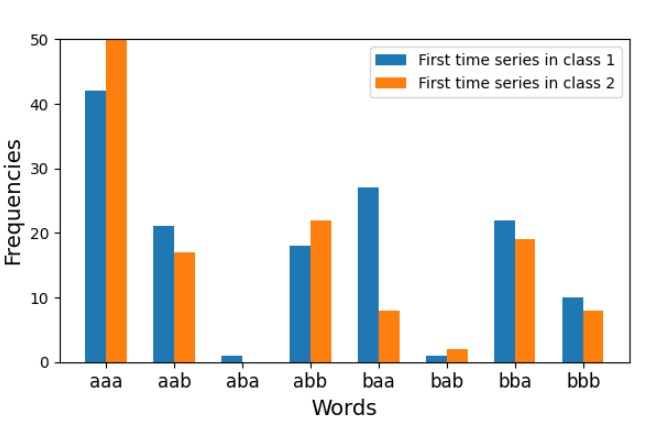
\includegraphics[width=0.8\textwidth]{images_ts/bag_of_patterns_adjusted.jpg}
    \caption{ Each time series is transformed into bag of words by  algorithm bag-of-patterns. The algorithm then calculates the frequencies of each word for each time series\cite{bag_of_patterns_img}.}
    \label{fig:bag_of_patterns}
\end{figure}

There exists an improvement to the above approach. It is called SAXVSM. 

\begin{itemize}
		\item The first difference is the way the time series is handled. With a help of a sliding window we get the subsequences of the time series. These subsequences are further standardized and normalized.
		\item The second difference is the way of evaluating the similarity of the time series. Algorithm uses adjusted version of TF-IDF which is used in many NLP tasks. It creates a TF-IDF matrix. The matrix has in rows the words that occur in the dataset, in columns are the classes that we have to classify. It is important to normalize the occurrence of a word over all of the classes in which it occurs.This step will give us the words specific to a particular class. 
	\end{itemize}

\subsubsection{Discretizing Fourier coefficients}
The algorithm works similarly to the raw time series discretization. The difference is that we work with the Fourier coefficients and not directly with the measured values of the time series. To discretize the information we use the symbolic Fourier approximation (SFA) \cite{symbolic_fourier_approximation}.

At the input of the algorithm we have a time series. First we get the coefficients of this time series using the discrete Fourier transform. When selecting the coefficients for further processing we have the following choices.

\begin{itemize}
		\item Supervised task -- if we solve the problem using supervised learning, we select Fourier coefficients that represent lower frequencies. These capture the trend and slower changes in the time series.
		\item Unsupervised task -- if we solve the problem in an unsupervised way, we always select one Fourier coefficient which is common for a larger number of time series from the dataset. For the selected coefficient we compute the F-statistic. We can also select the coefficients of higher series as final candidates. The condition is that they have a larger variance. It is assumed that a larger variance is positively correlated with the amount of information.
	\end{itemize}

It is important that the same coefficients are selected for all time series. here we can imagine data as a matrix. The rows are formed by the individual time series. The columns are the coefficients of the Fourier transform.

After creating the matrix, we need to discretize the coefficients of the Fourier transform. When discretizing, we have two choices. We use a uniform bin distribution in case our problem is supervised. In case the task is unsupervised, we gain the number of bins by entropy minimization. Here the principle is very similar to the creation of a decision criterion for node in a decision tree.

The adaptation will ensure that we get a time series represented by a single word. This approach is used in the \cite{BOSS} algorithm BOSS.

The most frequently used algorithm for preprocessing the time series is an extended version of Bag-of-SFA. The algorithm sequentially selects subsequences from the time series which are then discretized using SFA. We get a word from each subsequence. Then, for each time series, a histogram of word counts is produced. The preprocessed data is further classified using nearest neighbours classifier.

There are implementations that improve the base version of the algorithm. Their improvement consists of a similar idea as in the case of SAXVSM. The result is a TF-IDF matrix whose rows are individual sequences and columns represents classification classes.

\subsection{Ensemble models}
Using multiple models is meta in the world of machine learning. Time series classification is no exception in this respect. In the classical world of ensamble methods, each classifier belongs to a class of similar algorithms. For example, a random forest consists of a large number of decision trees.
In the case of the ensamble approach, the variance in accuracy is reduced because the model is composed of several independently trained models.

Recently created ensamble models include
\begin{itemize}
		\item The Collective of Transformation-Based Ensembles (COTE) which combines 35 classifiers of which 11 classifiers work with similarity of whole time series, 8 classifiers with shaplet transformation, 8 work with autocorrelation features and 8 with power spectrum.
		\item The Hierarchical Vote Collective of Transformation-Based Ensembles (HIVE-COTE) is an improved version of the previous COTE. It uses 2 new classifiers of BOSS and time series forest type and a new type of spectral classifier Random Interval Spectral Ensamble. The decision model is based on boosting. The decision of each classifier is assigned a weight based on its success rate in the cross validation process.
	\end{itemize}

\clearpage
\subsection{Markov transition field}
The method is based on the philosophy of the first order Markov chains. It is one of the algorithms that preprocess the time series. This preprocessed information can be further analysed or directly used as input to the model.
The first step of the method is to create $M$ quantiles by which the time series will be discretized. Each value of the time series $x_k$ belongs to a certain bin $m_i$. The algorithm is based on the idea that we can describe a probabilistic transition between any pair of bins $(m_i,m_j), \forall i,j \{1,\dots,M\}$. This creates a transition matrix. To form a Markov transition matrix, we need to ensure that the rows are normalized to represent a probability distribution.

Markov transition field then looks like
\[
MTF = \begin{bmatrix} 
    P(m(x_1)|m(x_1)) & \dots & P(m(x_1)|m(x_n)) \\
    \vdots & \ddots & \vdots \\
    P(m(x_n)|m(x_1)) & \dots  & P(m(x_n)|m(x_n)) 
    \end{bmatrix}
\]


where $m$ is a function that maps values from time series into one of $M$ bins, $P$ is a probability function and $n$ represents the length of time series. 

This solution has a few disadvantages
\begin{itemize}
		\item Its main disadvantage is that the matrix can be quite large. This problem can be solved by applying average pooling to the MTF matrix. This creates a matrix that has a smaller dimension.
		\item When using the MTF matrix we know the transition probabilities but we lose the time information when the transition occurred.
	\end{itemize}

The time series preprocessed by the MTF can serve as input for a convolutional neural network that takes care of the classification.

\begin{figure}[ht!]
    \centering
    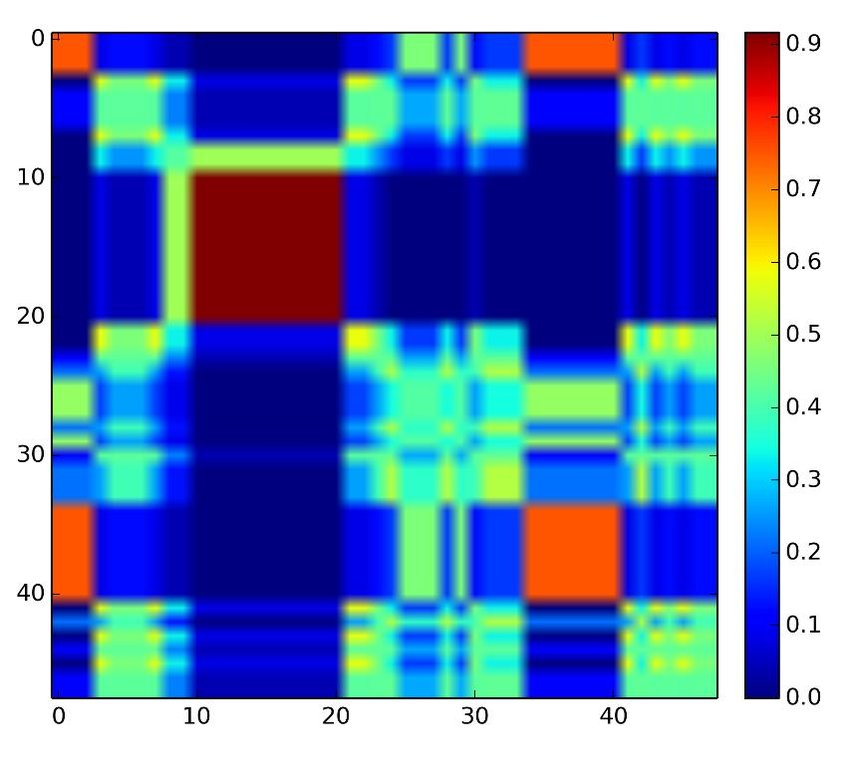
\includegraphics[width=0.8\textwidth]{images_ts/Markov_transition_field.jpg}
    \caption{Graphical representation of Markov transition field.}
    \label{fig:graphic_markov_transition_field}
\end{figure}


\clearpage
\subsection{Deep learning}
\subsubsection{Echo state architecture}
RNN architectures are used to work with time series. Nevertheless, they have their limitations and weaknesses.

The first one is duration of training. The input of the cell depends on the output of the previous recurrent cell. Therefore, such a process is very difficult to parallelize. RNN are most of the time train on CPUs and can not efficently utilize the many times faster GPUs.

The second problem is with vanishing gradients \cite{echo_state_network_paper}. The creators of the LSTM architecture tried to deal with this problem but it never goes away completely. What almost sidelines the LSTM architecture in our solution is the fact that we work with sparse data. With data in which the observed variable has many zero values, the vanishing problem is amplified.

For these reasons, an concept of echo state network was created so that it addresses and solves the problem of vanishing gradients to some extent.

\begin{figure}[ht!]
    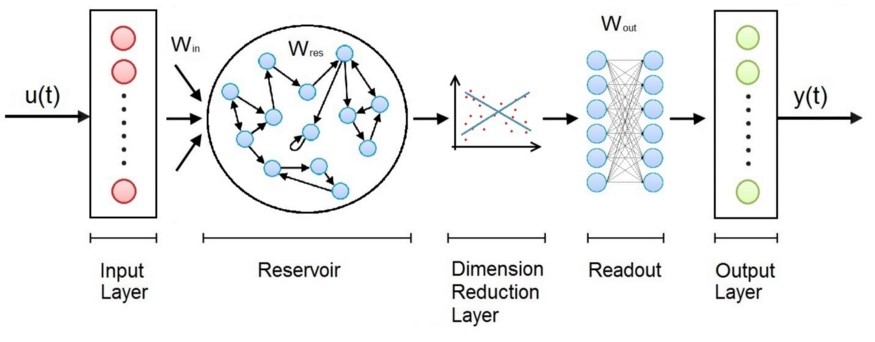
\includegraphics[width=1.0\textwidth]{images_ts/echo_state_network.jpeg}
    \caption{Echo state network \cite{time_series_classification}. } 
    \label{fig:echo_state_network}
    \centering
\end{figure}

The reservoir is the main part of the whole \cite{echo_state_network_reservoir} architecture. The reservoir is formed by an undirected graph where vertices represent RNN cells and edges are weighted connections between them. These weights are initialized as sparse and the vast majority of them have zero value so the connections between vertices are very sparse.

\noindent There are four types of weights used in the reservoir section
\begin{itemize}
		\item Input weights - connects the input layer and the reservoir.
		\item Output weights - connect the reservoir to the output layer, which serves as an input for the dimension reducing layer.
		\item Reservoir inner weights - are formed by sparse connections.
		\item Output weights -  they connect the output back to the reservoir and serve as a feed back.
	\end{itemize}
All of the reservoir weights are randomly initialized and remain static throughout the entire training.

The main role of the reservoir is to create a non-linear recurrent embedding. The data processed in this way is further used as input for the dimension reducing module. PCA is most often used.

Experiments \cite{echo_state_network_reservoir} showed that when the embedding dimension of the model is gradually reduced, the accuracy of the model decreases negligibly and the network training speed increases. The dimension reduction process has its lower bounded treshold. If we cross the treshold and dimensionality reduction becomes too restrictive then the PCA layer becomes a bottleneck for the architecture. After that, the accuracy decreases rapidly.

We can connect any type of network that is used for prediction after the dimensionality reduction module.

\subsubsection{Inception Time}
Models with derived architerture from InceptionNet are very successfully used in computer vision \cite{inception_net} tasks. The architecture itself has several versions. Gradually, as new papers came out, the Inception architecture was modified. 

The strength of the architecture lies in the variable lengths of the receptive field. For ordinary CNNs, the kernel size of the individual layers becomes a hyperparameter. The size of the receptive field densifies the information density that the NN can extract from the data. Smaller kernels tend to process local information well but miss the overall global picture. Kernels of larger sizes gain global information but lose local information because they have bigger receptive field \cite{inception_net}.

For Inception architecture, the authors decided to take advantage of good features from both worlds. The main idea of inception blocks is based on the use of several filter sizes in parallel. Then the output is concatenated. The next layer of the network chooses the information that is essential for minimizing the loss function. The filters in the inception block are often 1x1, 3x3, 5x5.

\begin{figure}[ht!]
    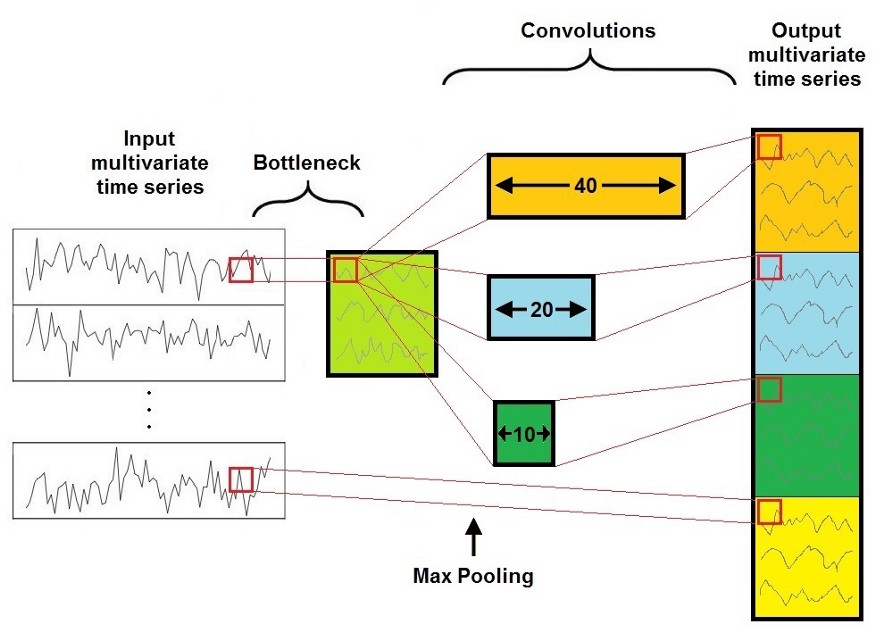
\includegraphics[width=1.0\textwidth]{images_ts/inception_time_block.jpeg}
    \caption{Block of inception time network} 
    \label{fig:inception_time_block}
    \centering
\end{figure}


\subsubsection{Architecture optimization}
Using the pooling layer, the network is able to change the size of the x, y dimension of the input data. However, it cannot efficiently aggregate information over the z-axis, which expresses the number of channels on the input layer or the number of filters on the layers inside the network. This problem has been solved very elegantly by using convolutive filters. In InceptionNet these are special 1x1 convolutional filters. These preserve the x,y dimensions of the input data with the same padding. Their main advantage is that they effectively aggregate the data along the z-axis. The number of mathematical operations during input processing is reduced without affecting the quality of the information \cite{one_one_conv}.

\begin{figure}[ht!]
    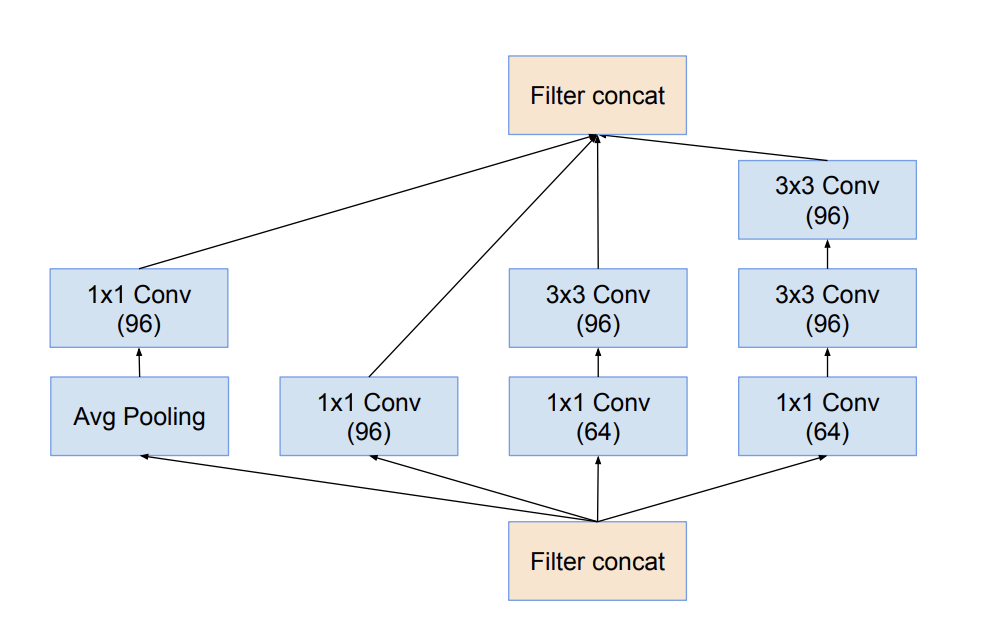
\includegraphics[width=1.0\textwidth]{images_ts/inception_block_conv1x1.png}
    \caption{Inception block in Inception V4 network. } 
    \label{fig:inception_block_onexone_conv}
    \centering
\end{figure}

Thanks to the use of 1x1 conv filters the data was processed into more compact blocks, which made the training of single inception blocks faster.

\subsubsection{Residual connections}
In newer versions of Inception architecture, the authors introduced the use of residual connections \cite{resnet_cnn}. 
The ability to capture information from the data is conditioned proportionally by the size of the model. Therefore the larger models are able to learn more. This is at least true in theory. Practice is a bit different. Without the use of residual connections, a very complex model with a large number of parameters will be worse in accuracy than a moderately sized model. 

In the process of back propagation, the strength of the gradient signal may gradually weaken until it completely disappears. This is a well-known problem. In order to avoid similar problems, we have to implement residual links in the network. This will create skip connections and the gradient signal will travel more efficiently through neural network during back propagation \cite{resnet_cnn}.

\chapter{Implementation}
\label{label:Implementation}
In the following chapter we discuss the design of the solution, its implementation, and the suitability of the individual approaches. We discuss the architecture of the used models. There is a comparison between these models and discussion  about the steps that led to the successful training. A part of the chapter is devoted to finding the right hyperparameters and the overall design of the training procedure. At the end of the chapter we present the results obtained.

\section{A path of implementation}
In the theoretical part we have discussed algorithms and approaches that could solve such a problem. We have described shaplet search, DTW, kernel methods, etc. Each of them has it`s own strengths and weaknesses (length of input, speed of processing, interpretation of decisions, etc.) In this work we decided to continue with deep learning models. 
\section{Working environment}

At first we concentrated on working on the local machine. Support scripts were created to retrieve information about the repositories. The information we needed to retrieve was only available through GithupAPI. Therefore, we needed to create a set of scripts that would allow us to do this. The information was related to the content of the subfiles, subfile types, etc. 
In this part of the development, a local machine with a virtual environment was a suitable solution.

Gradually we moved to the task of classifying the lifetime of the repository. We needed to process the dataset and train the models. For this purpose, the local stand is no longer suitable. So we decided to use a product from Google Research, Google Colab.

Google Colab is an environment designed for experimentation and work of data scientists. In colaboratory notebooks, the entire machine learning pipeline can be defined. From data acquisition through data cleaning and preparation for training to the actual training and evaluation of models. A huge added value is the possibility to work with the command line. A developer can customize a notebook, install the newer version packages needed for the new model architectures, experiment and return to a clean instance the next day.

Another reason why we chose Colab is the availability of GPUs. We wanted to experiment with larger models that require higher GPU performance and memory.

\section{Data generator}
As we mentioned in the \ref{label:training_data_generator} chapter, we have created a keras generator which is adapted for training large models. This generator can be used to train huge models that are loaded on multiple GPUs. Then the communication between GPUs and the synchronization of gradients becomes the bottleneck. There are technologies such as Horovod that try to overcome these problems.

In our solution, the generator was used for adaptive data augmentation. During the experiments we could choose what type of repository we consider inactive. 

\section{Problem analysis}
We took into account several key factors during the analysis and the following preparation of the models. 

First we had to estimate the size and complexity of the problem. The necessary complexity of the models and the architecture used depend on these metrics. 

This was followed by prototyping the simplest possible model. We wanted to achieve the following. The more generic the model is, the easier it is to modify it in case we want to use a more exotic architecture (for example combine LSTM and CNN).

Another useful feature of such a model is the speed of iteration through different solutions. When training a model on the same dataset, a model that has fewer parameters or less complicated architecture can be retrained faster. 

Another critical factor is the size of the dataset. When working with a large dataset, an end-to-end model learning approach is the best. The model captures the structural information contained in the data and does not need almost any humen expert knowledge to train the model. If we work with small dataset we often cannot use deep learning. The dataset does not contain enough information to train the model. Then we have to resort to more statistical methods (ARIMA, SARIMA, etc.) and rely on our expertise.

It can happen that despite a relatively simple model, the training process takes a long time and we cannot iterate fast enough. The problem may be with the size of the dataset. In our case we did not have to shrink the dataset. For example, if we worked with a very large dataset, we would have decreased its size. It is very reasonable to choose a smaller dataset that is as representative as possible and experiment with it.

When training, it is very important to find out whether the model we have created is able to capture the information in the dataset. This can be conditioned by the number of model parameters, the architecture used or the size of the dataset itself. In our case, we did not know what approaches would be the best to analyse the time series because the final dataset was quite small. There was still a possibility that deep learning approach could fail. Then we would have to analyzed data using other methods mentioned in \ref{label:Timeseries_classification}. We built simple deep learning models and tried to overfit the models on the adjusted data. 

Overfit on data becomes a rather good indicator that the size of the model and its architecture can approximately capture the complexity of the information from the dataset. We can then work with generic models and improve their accuracy.

We decided to use smaller models for gradual improvement because we had relatively little data that was very specific and we needed to iterate quickly.

\subsection{Models used during training}

In \ref{label:Timeseries_classification} we discussed algorithms and approaches that could solve such a task. We described shaplet searching, DTW usage, kernel methods, etc. Each of the approaches has something to offer. There are strengths and weaknesses of each (input length, processing speed, decision interpretation, quality of results, etc.).


In this work we decided to create 2 models. The first model is based on technology. Such models are often used in time-dependent data processing. As we will see next, LSTM based model had a problem and did not achieve sufficient accuracy, so we decided to implement another model. The second one is a CNN where we initially created a simplified inception block. The network became larger but the accuracy was not affected by this improvement. We decided to replace the inception blocks with a simpler architecture where we added a number of 1x1 convolutional filters.

\section{Training}
\label{label:training}
The first model to be trained was LSTM. We had the assumption that LSTM could be a good choice since we work with time series. After several changes of the model architecture and searching for hyperparameters, the results hardly improved. This suggested that LSTM might not be the right choice for this type of data.

This may be due to the nature of the data. As we discussed in chapter \ref{label:Dataset}, the data contains a large number of zero values. This problem could be solved using Croston's method which is designed to predict time series with intermittent events. 

As a possible alternative, we have constructed a convolutional network. Its huge advantage was relatively fast training compared to LSTM. It also achieved higher accuracy using a similar number of parameters as LSTM.


Both models assume a sufficiently large dataset on which the models can learn efficiently. 
In case we work with a smaller dataset, the deep learning approach cannot be used. None of the models would be able to achieve reasonable results. In that case we would need to choose more standard approaches \ref{label:Timeseries_classification}.

\subsection{Model training}

During the training process, we had to create models capable of classifying the time series from generic and almost non-functional models. During the whole process we followed the basic principles of hyperparameter tuning.

We have chosen an orthogonal approach. We fixed a set of parameters, manipulated one parameter and observed how such a change affects the accuracy of the model. The most important parameter, which was mainly related to data preprocessing, was how many months must have passed since the last commit for the repository to be considered inactive. It turned out that the most accurate value is 12 months.

When working on the models we experimented with the size of the batch. We standardized the data and compared the accuracy against the raw unadjusted data. 


We applied a batch normalization layer just after the activation functions which solves the covariance. This is a phenomenon where the activation functions from the previous layer project data in a shifted distribution. As a consequence, the next layer works with information that is not standardized and suffers from a worse \cite{batch_normalization} gradient transition during back propagation.

We experimented with the size of the individual models, where we proportionally increased the number of parameters in the layers with respect to the base line model to see if this has an effect on the accuracy.

In the case of regularization, we had to approach each model separately. For LSTM we decided for a very fine L2 regularization because the model had a problem to achieve reasonable results and it has no problem with overfit. In case of CNN, we quickly encountered a problem with overfitting and we had to use a dropout after each convolutional layer. Especially for CNN architecture this decision had a significant impact on the final accuracy.

A great help during training and evaluation of models is the use of confusion matrix. This way we can see the correctly classified data and we can also discover where the problem is.
The accuracy of the individual models increased when we decided to approach the task as a multivariate time series classification.
Then the information can be spread across several time series.

\section{Loss function}
We decided to use the categorical cross entropy as a loss function. Such a function was a great fit because the target variable was transformed into one hot vector.
\begin{equation*}
    loss_{CE} = - \sum_{i=1}^{c}y_i \cdot log (\hat{y_i})
\end{equation*}

where $\hat{y_i}$ is the value on index i in vector $\hat{y}$, 
$y_i$ is the corresponding target value on index i in vector $y$ and output size is the number of classes.
\newpage
\section{Results}
\subsection{Long short term memory}

LSTM had a hard time getting past a certain threshold during training. We assume that this was due to the nature of the dataset. To confirm this assumption, we trained the model on information aggregated by day, week and month. The smaller the aggregation window, the more zeros in the dataset. Models trained on daily and weekly aggregations were significantly more inaccurate than models trained on monthly aggregations.

While training and tunning the hyperparameters we had to solve a few problems. The accuracy of the model was not sufficient and so we decided to train an alternative model. This decision turned out to be correct. We were able to create a CNN model with a relatively high accuracy.

\subsection{Instability during training}
We have tried to solve this problem by gradually reducing the size of the learning rate. The solution helped only partially. In case we used a low learning rate, the network hardly converged. We were forced to use a gradual decrease of the learning rate followed by a restart. Even this method did not ensure that the network converged to a higher accuracy.
 

\subsection{Insufficient accuracy}
We tried to solve the problem by adding more memory cells in the recurrent layer, extending the network, adding parallel dense layers.
\begin{itemize}
		\item The increased number of memory cells in LSTM layers affected the overall result and the training process very slightly. It almost did not solve the problem with relatively large variance during convergence of training and validation error.
		\item Proportionally rescaled network only took longer to train. With almost no effect on overall training process.
		\item By adding parallel dense layers, we tried to introduce absolute information about the maximum or minimum activity in the data. Even this improvement did not show an increase in validation accuracy.
	\end{itemize}

Despite all attempts we could not train the model to achieve higher accuracy. Regardless of the improvements we made to the network, the training process hit the upper threshold and we could not overcome it. 


\begin{figure}[ht!]
    \centering
    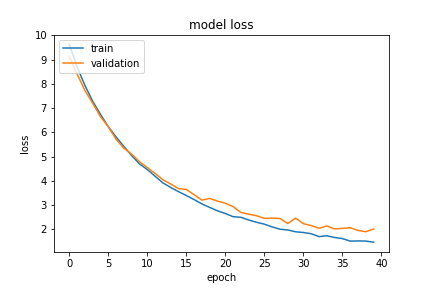
\includegraphics[width=0.75\textwidth]{images_ts/loss_LSTM.png}
    \caption{Loss function progress for LSTM}. 
    \label{figure:lstm_loss}
    \centering
\end{figure}

\begin{figure}[ht!]
    \centering
    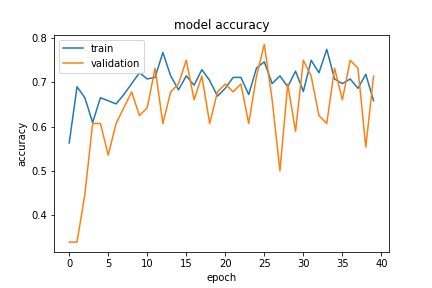
\includegraphics[width=0.75\textwidth]{images_ts/accuracy_LSTM.png}
    \caption{Accuracy function progress for LSTM}. 
    \label{figure:lstm_acc}
\end{figure}

\clearpage
\subsection{Convolutional neural network}
The convolutional neural network was created as an alternative architecture. We suspected that LSTM does not achieve the desired results because we are working with quite specific data.

Convolutional neural network did not access the data as sequential time-dependent information.
For the first convolution models we were inspired by the Inception architecture. Its blocks were too big and unnecessarily too complicated. In first designs of the network, we used inception blocks that were smaller. In the end we decided to omit the inception blocks altogether.
When designing the model we decided to keep mainly 1x1 convolution filters. This decision turned out to be the right one, which can be seen in the validation results. 

At the beginning we worked only with information from one time series.
When we switched to multivariate task, we modified the models slightly.

\begin{figure}[ht!]
    \centering
    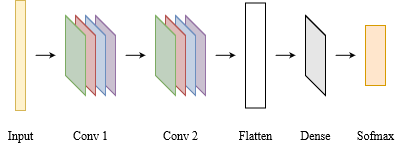
\includegraphics[width=0.75\textwidth]{images_ts/Diagram_cnn.png}
    \caption{High level architecture of CNN. Each convolution block consists of convolution filter, batch normalization, dropout and maxpooling}. 
    \label{figure:cnn_diagram}
    \centering
\end{figure}

\subsection{Better results}
We could see even during initial experiments that the training and validation errors converge to better results than LSTM. This may be caused by a different data access. CNN does not contain memory cells and did not suffer when there were many zeros on the time series segment. The overall accuracy of the final model is 15\% higher than the accuracy of the LSTM \ref{figure:cnn_acc}.

\begin{figure}[ht!]
    \centering
    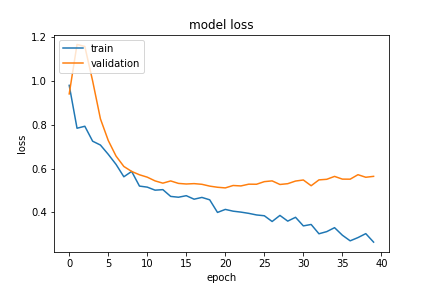
\includegraphics[width=0.75\textwidth]{images_ts/loss_CNN_graph_good.png}
    \caption{Loss function progress for CNN}. 
    \label{figure:cnn_loss}
    \centering
\end{figure}

\begin{figure}[ht!]
    \centering
    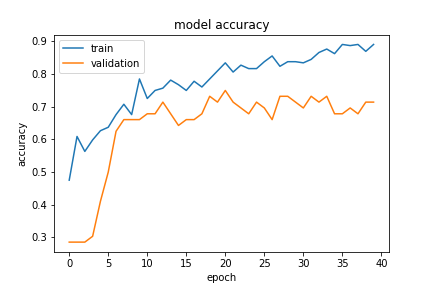
\includegraphics[width=0.75\textwidth]{images_ts/accuracy_CNN_graph_good.png}
    \caption{Accuracy function progress for CNN}. 
    \label{figure:cnn_acc}
\end{figure}


The training process was much more systematic. At the beginning we tried to get an architecture that can overfit on data. Then we tried to regularise the model. Since we worked with convolution filters, the training time was an order of magnitude less than with LSTM.

\section{Model accuracy}
When creating the models we started with more generic architectures and gradually moved towards more specialized ones. This is true for both LSTM and CNN. Then we tried to improve the architecture, find more suitable hyperparameters, change the learning rate, etc. These steps are described in chapter \ref{label:training}.


\begin{table}[!ht]\centering
    \begin{tabular}{l|c}
         \textbf{Network achitecture} & \textbf{accuracy} \\\hline\hline
         LSTM & 0.72\\
         CNN & \textbf{0.86}\\
    \end{tabular}
    \caption{Classification accuracy on validation dataset.}
    \label{tab:bigger_models}
\end{table}

We decided to measure the final accuracy of the CNN on the test data. its accuracy is 87\%.

We know from theory that the accuracy on test set should be slightly lower than on validation set. The fact that it is higher may be due to smaller test set where the dataset distribution is not exactly the same as the validation one. With smaller datasets this can happen.

\chapter{Conclusion}
Developers nowadays rely on many libraries and tools that they use as a ready-made solution when creating a new project. The requirement is that these 3rd party libraries serve as a tool during product development. Most of the time there is not just one library which can solve the problem but few of them. Then the team needs to choose one that best fits the team's requirements and criteria. In this work, we have been exploring the possibilities of using machine learning models to estimate the lifetime of a repository.

The main objective of the theoretical part was to define the concepts from the theory that we work with during the thesis. In the theoretical part we further described the basic properties of time series. This information is mentioned in \ref{label:Time_series_introduction}.

In chapter \ref{label:Timeseries_classification} we created an exhaustive overview of algorithms used for working with time series. We analyzed each of them in detail. We discussed its functioning, its weaknesses and strengths, and possible extensions. In deep learning part, we introduced reader to models designed for processing time series. Here, we looked in depth  at two different architectures.

Chapter \ref{label:Useful_tools} is devoted to the analysis of tools usable for obtaining a dataset or a part of it. Most of the tools tested during the work on the thesis were not suitable. None of them could be used as a stand alone solution. That is why we decided to combine them. We used the best of several worlds.

In sections \ref{label:Exploratory_data_analysis} and \ref{label:Dataset} we also discussed the dataset acquisition and preparation. We suggested what attributes to use and how to prepare the data, taking into account its specific character.

In the practical part \ref{label:Implementation} we dealt with described training process. We explored deep learning approaches to solve the problem. We dealt with the analysis of training and validation graphs. We look at the problems we solved during training. We evaluate the accuracy of the models.

Based on the obtained results, we can conclude that a convolutional network with the proposed architecture can indeed predict the lifetime of the repository quite accurately.

\section{Outline of future work}
A further step to improve the classification accuracy is to obtain more data. While preprocessing the dataset we had to discard many repositories. In this regard, we would need to communicate with the GithubAPI team as the download speed was a very limiting factor. Another alternative is to use a library that supports such massive data collection. 

An alternative way to improve classification accuracy is to create larger and more specialized models. Larger models with a more comprehensive dataset would probably produce better results.

Trained models are only one part of the solution. If we wanted to analyse the repository more comprehensively, we could analyse its contents. Such an analysis could be done for the whole files as well as for smaller parts or for individual functions. This would mean analyzing the files and examining the quality of the source code. Another possibility of extension is to focus on the analysis of used libraries and packages. This would allow us to identify those that contain potential vulnerabilities.

\printbibliography

\setsecnumdepth{all}
\appendix

\chapter{Acronyms}

\begin{description}
	\item[NN] Neural network
	\item[ML] Machine learning
	\item[DL] Deep learning
	\item[TS] Time series
	\item[DTW] Dynamic time warping
	\item[CNN] Convolutional Neural Network
	\item[RNN] Recurrent neural network
	\item[LSTM] Long short term memory
	\item[GPU] Graphics Processing Unit
\end{description}

\begin{figure}
	\dirtree{%
		.1 readme.txt\DTcomment{the file with USB contents description}.
		.1 src\DTcomment{the directory of source codes}.
		.2 model\_weights\DTcomment{the directory with pretrained weights}.
		.2 models\DTcomment{the directory with model architectures}.
		.2 training\_utils\DTcomment{the directory with scripts needed for training}.
		.2 testing\_model\_weights.ipynb\DTcomment{notebook for testing models}.
		.2 utils\_notebooks\DTcomment{extract data from GithubAPI}.
		.2 dataset\_preprocess.ipynb\DTcomment{steps to preprocess dataset}.
		.2 notebooks\_from\_github.ipynb\DTcomment{ access to GithubAPI}.
		.2 training\_models\DTcomment{training and validating}.
		.1 text\DTcomment{the thesis text directory}.
		.2 fig\DTcomment{the directory with figures}.
		.2 ref.bib\DTcomment{the bibliography resource}.
		.2 thesis.pdf\DTcomment{the thesis text in PDF format}.
		.2 thesis.tex\DTcomment{the thesis text in LATEX format}.
	}
\end{figure}

\end{document}
